En esta sección se detallan los experimentos realizados para:
\begin{itemize}
    \item Validar si el modelo y la simulaciones sobre el mismo, logran caracterizar el comportamiento de la función \emph{Image Handler} en distintos escenarios. 
    \item Estudiar el comportamiento de la función Lambda cuando es invocada con cargas de trabajo y
    \item Comparar los resultados de las invocaciones de la función Lambda con los de la herramienta SAM CLI.
\end{itemize}

\subsection{Utilizando \emph{Image-Handler} para redimensionar imágenes de distintos tamaños} \label{sec:experimento-1}
%Este es el caso que se menciona en la Sección \ref{sec:manejador-imagenes-spe} y se muestra en la figura \ref{fig:serverless-image-handler-architecture-workflow}. Se probó la función Lambda con dos imágines: una de tamaño pequeño ($\sim$100Kb) y otra de tamaño grande ($\sim$5Mb). El objetivo es comprobar cómo los distintos tamaños de las imágenes influyen en el tiempo de respuesta de la función.

Este es el caso que se menciona en la Sección \ref{sec:manejador-imagenes-spe} y se muestra en la figura \ref{fig:serverless-image-handler-architecture-workflow}. Se realizaron invocaciones a la función Lambda con tres grupos de imágenes:
\begin{enumerate}
    \item Imágenes de tamaño menor o igual a 500Kb.
    \item Imágenes de tamaño mayor a 500Kb y menor a 1Mb.
    \item Imágenes de tamaño mayor a 1Mb y menor a 2Mb.
\end{enumerate}
En este experimento, el objetivo es comprobar por medio de mediciones directas y de simulaciones en un modelo, cómo los distintos tamaños de las imágenes influyen en el tiempo de respuesta de la función.

Intuitivamente, se espera que, cuando se hagan solicitudes de redimensionamiento de imágenes de mayor tamaño tomen mayor tiempo en ser procesadas y que lo contrario suceda con las imágenes de menos tamaño. Los resultados obtenidos brindan una referencia inicial para saber cómo es que los componentes de software asociados al redimensionamiento trabajan y qué posibles mejoras podrían realizarse.

Las cargas de trabajo para este experimento son de tipo \emph{cerrada}, lo que quiere decir que una solicitud se ejecuta solamente hasta que la anterior se termina. Esto va orientado a tener mejor trazabilidad de lo que ocurre con la función.

%%%%%%%%%%%%%%%%%%% 1

\subsubsection{Invocaciones con imágenes menores a 500Kb}
Para la realización de este experimento se contó con la siguiente configuración base:
\begin{itemize}
    \item \emph{Sujeto de prueba:} La función Lambda IM-Simple.
    \item \emph{Repositorio de imágenes:} \emph{Cluster} de 1000 imágenes de tamaño menor a 500Kb alojadas en Amazon S3.     
    \item \emph{Carga de trabajo:} 1000 invocaciones secuenciales de redimensionamiento de imágenes con dimensiones aleatorias a IM-Simple.
    \item \emph{Herramientas de medición:} Amazon Cloudwatch.
\end{itemize}

Configuración para la obtención de datos de rendimiento

\begin{itemize}
    \item \emph{Sujeto de prueba:} Las funciones Lambda IM-KP y IM-XRay
    \item \emph{Repositorio de imágenes:} \emph{Cluster} de 1000 imágenes de tamaño menor a 500Kb alojadas en Amazon S3.     
    \item \emph{Carga de trabajo:} 1000 invocaciones secuenciales de redimensionamiento de imágenes con dimensiones aleatorias a IM-PK y IM-XRay.
    \item \emph{Herramientas de medición:} Kieker, PMX y Amazon X-Ray.
\end{itemize}

Para la realización de este experimento, se obtuvieron 1000 imágenes aleatorias de tamaño menor a 500Kb del servicio \emph{Lorem Picsum}\footnote{\url{https://picsum.photos}}. Se creó un \emph{script} en \texttt{Bash} para acceder a la interfaz de programación (API) proporcionada por \emph{Lorem Picsum} para descargar de forma aleatoria 1000 imágenes cuyo tamaño era menor a los 500Kb. La distribución del tamaño de las 1000 imágenes, en Kb, se aprecia en la figura \ref{fig:distribucion-tamanno-imagenes-hasta-500kb}. El mismo grupo de imágenes se utilizó para realizar solicitudes de redimensionamiento sobre IM-Simple, IM-KP y IM-XRay.

\begin{figure}
\hspace{-1cm}
\begin{tikzpicture}
\begin{axis}[
  width=15cm, height=10cm,
  title={\textbf{Distribución del tamaño de imágenes de tamaño $\leq 500Kb$}},
  ylabel={\small Cantidad de imágenes},
  x label style={at={(axis description cs:0.5,-0.1)},anchor=north},
  xlabel={\small Tamaño de las imágenes (En $Kb$)},
  xmin=0, ymin=0, xmax=550,
  ybar interval,
  xtick=data,
  xticklabel interval boundaries,
  x tick label style={rotate=30,anchor=east}
  ],
	\addplot+[hist={bins=10}]
		table[col sep=comma, y index=0] {datos/tamannos-cluster-a.csv};
\end{axis}
\end{tikzpicture}
\caption{Distribución del tamaño de imágenes $\leq 500Kb$}
\label{fig:distribucion-tamanno-imagenes-hasta-500kb}
\end{figure}

\paragraph{Medición Base: 1000 invocaciones de redimensionamiento de imágenes en IM-Simple.} 
Se creó un \emph{script} en \texttt{Bash} para ejecutar 1000 invocaciones de redimensionamiento en la función IM-Simple en las imágenes de tamaño menor a 500Kb. El \emph{script} selecciona una imagen de forma aleatoria y luego ejecuta la solicitud de redimensionamiento utilizando dimensiones de ancho y alto de uso común para imágenes en miniatura (\emph{thumbnails}) \textbf{AGREGAR APARTADO SOBRE LA ELECCION LOS THUMBNAILS}.

\begin{figure}[h]
\hspace{-1.0cm}
\begin{tikzpicture}
\begin{axis}[
  width=16cm, height=8cm,
  title style={align=center},
  title={\textbf{Distribución de los tiempos de respuesta en solicitudes de redimensionamiento}\\\textbf{de imágenes de tamaño $\leq 500Kb$ en IM-Simple}},
  ylabel={\small Solicitudes de redimensionamiento},
  x label style={at={(axis description cs:0.5,-0.21)},anchor=north},
  xlabel={\small Tiempos de respuesta (En $ms$)},
  xmin=0, ymin=0, xmax=4020,
  ybar interval,
  xtick=data,
  xticklabel interval boundaries,
  x tick label style={rotate=30,anchor=east}
  ],
	\addplot+[fill=red!70!white,hist={bins=10}]
		table[col sep=comma, y index=0] {datos/tiempos-de-respuesta-hasta-500kb-simple.csv};
\end{axis}
\end{tikzpicture}
\caption{Distribución de los tiempos de respuesta en solicitudes de redimensionamiento de imágenes de tamaño $\leq 500Kb$ en IM-Simple}
\label{fig:distribucion-solicitudes-imagenes-hasta-500kb}
\end{figure}

\begin{figure}[h]
%\vspace{-4cm}
\hspace{-1.0cm}
\begin{tikzpicture}
\begin{axis}[
  width=16cm, height=8cm,
  title style={align=center},
  title={\textbf{Distribución de los tiempos de respuesta en solicitudes de redimensionamiento}\\\textbf{de imágenes de tamaño $\leq 500Kb$ en las simulaciones de Palladio}},
  ylabel={\small Solicitudes de redimensionamiento},
  xmin=0, ymin=0, xmax=4000,
  ybar interval,
  xtick=data,
  x label style={at={(axis description cs:0.5,-0.2)},anchor=north},
  xlabel={\small Tiempos de respuesta (En $ms$)},  
  xticklabel interval boundaries,
  x tick label style={rotate=30,anchor=east}
  ],
	\addplot+[hist={bins=10}]
		table[col sep=comma, y index=0] {datos/tiempos-de-respuesta-hasta-500kb-palladio.csv};
\end{axis}
\end{tikzpicture}
\caption{Distribución de los tiempos de respuesta en solicitudes de redimensionamiento de imágenes de tamaño $\leq 500Kb$ en las simulaciones de \emph{Palladio Workbench}}
\label{fig:distribucion-simulacion-imagenes-hasta-500kb}
\end{figure}

En la figura \ref{fig:distribucion-solicitudes-imagenes-hasta-500kb} se muestra la distribución de los tiempos de respuesta en las solicitudes de redimensionamiento en las imágenes de tamaño menor a 500Kb. Con excepción de la primera invocación, la cual tuvo una duración de 4 segundos, más del 97,5\% de las invocaciones no superó los 1,6 segundos.

\paragraph{Mediciones para obtención de modelo de rendimiento: 1000 invocaciones de redimensionamiento de imágenes en IM-PK y IM-XRay.} Se utilizó el mismo \emph{script} en \texttt{Bash} y la misma configuración para generar invocaciones a la función Lambda descrita en la sección anterior.

En primera instancia se ejecutaron 1000 invocaciones a IM-PK para generar una bitácora de Kieker y a partir de la misma extraer un modelo de rendimiento PCM usando PMX. Tal y como se señala en la Sección \ref{sec:image-handler-xray}, las estimaciones hechas por PMX sobre el rendimiento de los componentes del modelo se basaban en valores constantes. Fue por esta razón que, para contar con una versión alternativa de \emph{Image Handler} que pudiera brindar otro nivel de detalle en las  métricas de rendimiento, se introdujo IM-XRay.

Al igual que en caso anterior, se ejecutaron 1000 invocaciones a IM-XRay, y por medio de un \emph{script} en \texttt{Bash}, se obtuvieron las trazas correspondientes a las 1000 invocaciones. Los nuevos datos fueron exportados a formato \texttt{.csv} e interpretados con el lenguaje \texttt{R}. En \texttt{R}, se calcularon distribuciones de frecuencia de la probabilidad en la que un componente lograba procesar una porción de la carga de trabajo total. Estos datos fueron incluidos en los \emph{SEEFs} de cada componente del modelo. Por último se ejecutó una simulación en \emph{Palladio Workbench} con los siguientes parámetros:
\begin{itemize}
    \item Generación de 1000 mediciones.
    \item Carga de trabajo: \emph{cerrada}. Se ejecuta una solicitud sobre el modelo hasta que la anterior termina. 
\end{itemize}

%\hspace{-4cm}
\begin{table}
    \centering
    \begin{tabular}{l|r|r|r}
        \toprule[1.5pt]
        \multicolumn{4}{c}{\textbf{Hasta 500Kb}} \\
        \midrule
        Solicitud de redimensionamiento  & IM-Simple & PCM & Diferencia\\
        \midrule
        Tiempo promedio  & 583.842ms & 793.808ms & 209.965ms\\
        Desviación estándar & 460.659ms & 465.441ms & 4.782ms\\
        Varianza & 212206.961 & 216635 & -- \\
        Mediana & 466.715ms & 680.482ms &. -- \\
        Coeficiente de variación & 0.987 & 0.683 & -- \\                       
        \bottomrule[1.5pt]
    \end{tabular}
    \caption{Resumen de datos estadísticos}
    \label{table:datos-estadisticos-hasta-500kb}
\end{table}

En la figura \ref{fig:distribucion-simulacion-imagenes-hasta-500kb}, se muestra la distribución de los tiempos de respuesta en las solicitudes de redimensionamiento en las simulaciones de \emph{Palladio Workbench} para imágenes de tamaño $\leq 500Kb$. En los resultados de las simulaciones, el 95\% de las invocaciones no superó los 1,6 segundos en procesar la solicitud de redimensionamiento.

En este punto, se cuenta con 1000 mediciones hechas sobre IM-Simple y un modelo al que se le simularon 1000 invocaciones. En la figura \ref{fig:comparacion-imsimple-palladio-500kb} se comparan los tiempos de respuesta obtenidos en IM-Simple y los de las simulaciones, y, en el Cuadro \ref{table:datos-estadisticos-hasta-500kb}, un resumen de los datos estadísticos de los tiempos de respuesta en ambos sujetos de prueba.

\begin{figure}[h]
\hspace{-1cm}
\begin{tikzpicture}
	\begin{axis}[
	width=16cm, height=12cm, xmin=0, ymin=0,
	xmax=1010, ymax=4500,
	title={\textbf{1000 Solicitudes de redimensionamiento de imágenes de tamaño $\leq 500Kb$}},
	xlabel={\small Número de ejecución de solicitud de redimensionamiento},
	ylabel={\small Milisegundos},
	grid=major, grid style=dashed, label style={font=\small},
%	extra y ticks={400,600},
%	extra y tick labels={PP, PIM},
   extra y tick style={%
     color=green,
    },	
	tick label style={font=\footnotesize},
	scatter/classes={%
		a={mark=square*,blue},%
		b={mark=square*,red},%
		c={mark=o,draw=black}}]					
	\addplot[scatter,only marks,%
		scatter src=explicit symbolic]%
	table[meta=label, col sep=comma] {datos/xy-data-hasta-500kb.csv};
	
	\legend{Simulaciones de Palladio, Solicitudes a IM-Simple}
	\end{axis}
\end{tikzpicture}
\caption{IM-Simple \emph{vs} simulaciones en PCM: 1000 solicitudes de redimensionamiento de imágenes de tamaño $\leq 500Kb$.}
\label{fig:comparacion-imsimple-palladio-500kb}
\end{figure}

\begin{figure}[h]
\hspace{-1.5cm}
\begin{tikzpicture}
\begin{axis}[
    width=16cm, height=12cm,
    title={\small \textbf{Probabilidad acumulada: solicitudes de redimensionamiento en imágenes $\leq 500Kb$ en PCM}},
    xlabel={\small Segundos},
    ylabel={\small Probabilidad acumulada},
    xmin=0, xmax=4.2,
    ymin=0, ymax=1.05,
    extra y ticks = {0.9,0.95},
    extra x tick style={tick label style={font=\footnotesize}},    
	legend style={at={(0.5,-0.15)},
		anchor=north,legend columns=-1},
    grid=major,
    grid style=dashed,
]

\addplot[mark=none,blue,smooth] table [col sep=comma] {datos/hasta-500kb-cdf.csv};

\coordinate (a) at (axis cs:1.6, 0.95);
\draw[blue, dashed, thick](a |- current plot begin) -- (a);
 
\end{axis}
\end{tikzpicture}
\caption{Probabilidad acumulada en solicitudes de redimensionamiento en imágenes de tamaño $\leq 500Kb$ en \emph{Palladio Workbench}}
\label{fig:funcion-acumulada-palladio-500kb}
\end{figure}

\subsubsection{Análisis de resultados} 
La Figura \ref{fig:comparacion-imsimple-palladio-500kb} muestra un panorama alentador. Las ejecuciones de las simulaciones en PCM presentan tiempos de respuesta muy similares a los que entrega IM-Simple. Hay una diferencia de 209,965ms en el tiempo promedio de los tiempos de respuesta de las simulaciones en PCM con respecto a los tiempos de IM-Simple. Preliminarmente, se valora que, debido a que la versión IM-XRay tiene activado el servicio de monitoreo AWS X-Ray y que fue esta versión de \emph{Image Handler} utilizada como referencia para generar los tiempos procesamiento estimados para cada componente del modelo, instrumentalizar la función Lambda con el servicio de monitoreo AWS X-Ray genera un costo adicional (\emph{overhead}) en el procesamiento de la función. Cabe mencionar que la estrategia de monitoreo utilizada fue muy agresiva, pues para obtener nuevas métricas para los componentes del modelo PCM, se habilitaron muchos puntos de monitoreo dentro del código fuente. Además, se configuró la función Lambda para que monitoreara el 100\% de las invocaciones a solicitudes de redimensionamiento. Esta configuración de monitoreo no es la habitual que se utiliza para las funciones Lambda en producción, pero, para el caso de este estudio se necesitó contar con mayores niveles de detalle en las mediciones por lo que fue necesario sacar el mayor provecho al monitoreo. Mientras menor sean utilizadas las opciones de monitoreo de AWS X-Ray en la función Lambda, menor será el \emph{overhead} experimentado, tal y como pasa con IM-Simple en donde no se experimenta \emph{overhead} por concepto de monitoreo.

Los resultados muestran desviaciones estándar de 460,569ms y 465,445ms para IM-Simple y las simulaciones de PCM respectivamente. La desviación estándar de las simulaciones de PCM es solamente 4,782ms mayor que la de IM-Simple, lo que sugiere que la agrupación de los datos con respecto a su media aritmética serán muy semejantes.

Los coeficientes de variación para IM-Simple y las simulaciones de PCM fue de 0.987 y 0.683 respectivamente. Estos resultados apuntan a una mayor heterogeneidad entre los tiempos de respuesta y a que el tiempo promedio de procesamiento no se considere representativo para este conjunto de datos. Esta variabilidad viene dada por las diferencias de los tamaños de las imágenes utilizadas para este experimento, como se muestra en la Figura \ref{fig:distribucion-tamanno-imagenes-hasta-500kb}: imágenes de tamaño $\leq 500Kb$, en donde existen diferencias de hasta 500x, por lo que, por ejemplo, el tiempo de procesamiento de una imagen de tamaño de 5Kb será más rápido que una de tamaño de 490Kb.

Por último, de acuerdo con los resultados de las simulaciones, existe un 95\% de probabilidad de que el tiempo de procesamiento de una solicitud de redimensionamiento de una imagen de tamaño $\leq 500Kb$ tome 1,6 segundos o menos (Figura \ref{fig:funcion-acumulada-palladio-500kb}). En IM-Simple, se obtuvo un 97,5\% de probabilidad para el mismo caso (Figura \ref{fig:distribucion-solicitudes-imagenes-hasta-500kb}). Para este caso en particular y, debido a la variabilidad de los tiempos de respuesta, se considera que el uso de esta probabilidad acumulada es más representativa a la hora de describir el comportamiento de la función Lambda.

%%%%%%%%%%%%%%%%%%% 2

\subsubsection{Invocaciones con imágenes mayores a 500Kb y menores o igual a 1Mb}
Para la realización de este experimento se contó con la siguiente configuración base:
\begin{itemize}
    \item \emph{Sujeto de prueba:} La función Lambda IM-Simple.
    \item \emph{Repositorio de imágenes:} \emph{Cluster} de 1000 imágenes de tamaño mayor a 500Kb y menor o igual a 1Mb alojadas en Amazon S3.     
    \item \emph{Carga de trabajo:} 1000 invocaciones secuenciales de redimensionamiento de imágenes con dimensiones aleatorias a IM-Simple.
    \item \emph{Herramientas de medición:} Amazon Cloudwatch.
\end{itemize}

Configuración para la obtención de datos de rendimiento

\begin{itemize}
    \item \emph{Sujeto de prueba:} La función IM-XRay
    \item \emph{Repositorio de imágenes:} \emph{Cluster} de 1000 imágenes de tamaño mayor a 500Kb y menor o igual a 1Mb alojadas en Amazon S3.     
    \item \emph{Carga de trabajo:} 1000 invocaciones secuenciales de redimensionamiento de imágenes con dimensiones aleatorias a IM-XRay.
    \item \emph{Herramientas de medición:} Amazon X-Ray.
\end{itemize}

Para este experimento no se realizó ningún trabajo sobre la versión IM-KP porque no se necesita extraer ningún modelo. El modelo fue extraído y generado en el experimento anterior y debido a que se usa es el mismo código con los mismos puntos de monitoreo, un eventual proceso de extracción daría como resultado el mismo modelo del experimento anterior. Lo que sí fue necesario hacer, fue calibrar el modelo existente con los resultados de las mediciones a solicitudes de redimensionamiento en imágenes de tamaño mayor a 500Kb y menor o igual 1Mb, utilizando la versión IM-XRay. 

Para la realización de este experimento, se obtuvieron 1000 imágenes aleatorias de tamaño mayor a 500Kb y menor o igual a 1Mb del servicio \emph{Lorem Picsum}. Se ejecutó el \emph{script} en \texttt{Bash} del experimento anterior para acceder a la API de \emph{Lorem Picsum} para descargar de forma aleatoria 1000 imágenes cuyo tamaño fuera mayor a los 500Kb y menor o igual a 1Mb. La distribución del tamaño de las 1000 imágenes, en Kb, se aprecia en la figura \ref{fig:distribucion-tamanno-imagenes-hasta-1mb}. El mismo grupo de imágenes se utilizó para realizar solicitudes de redimensionamiento sobre IM-Simple y IM-XRay.

\begin{figure}
\hspace{-1.0cm}
\begin{tikzpicture}
\begin{axis}[
  width=15cm, height=10cm,
  title={\textbf{Distribución del tamaño de imágenes de tamaño $500Kb \leq x \leq 1Mb$}},
  ylabel={\small Cantidad de imágenes},
  x label style={at={(axis description cs:0.5,-0.2)},anchor=north},
  xlabel={\small Tamaño de las imágenes (En $Kb$)},
  xmin=0, ymin=0, xmin=500, xmax=1024,
  ybar interval,
  xtick=data,
  xticklabel interval boundaries,
  x tick label style={rotate=45,anchor=east}  
  ],
	\addplot+[hist={bins=10}]
		table[col sep=comma, y index=0] {datos/tamannos-cluster-b.csv};
\end{axis}
\end{tikzpicture}
\caption{Distribución del tamaño de imágenes $500Kb \leq x \leq 1Mb$}
\label{fig:distribucion-tamanno-imagenes-hasta-1mb}
\end{figure}

\paragraph{Medición Base: 1000 invocaciones de redimensionamiento de imágenes en IM-Simple.} 
Se ejecutó el \emph{script} en \texttt{Bash} del experimento anterior para ejecutar 1000 invocaciones de redimensionamiento en la función IM-Simple en las imágenes de tamaño mayor a 500Kb y menor o igual a 1Mb. El \emph{script} selecciona una imagen de forma aleatoria y luego ejecuta la solicitud de redimensionamiento utilizando dimensiones de ancho y alto de uso común para imágenes en miniatura.

\begin{figure}
\hspace{-1.0cm}
\begin{tikzpicture}
\begin{axis}[
  width=16cm, height=8cm,
  title style={align=center},
  title={\textbf{Distribución de los tiempos de respuesta en solicitudes de redimensionamiento}\\\textbf{de imágenes de tamaño $500Kb \leq x \leq 1Mb$ en IM-Simple}},
  ylabel={\small Solicitudes de redimensionamiento},
  x label style={at={(axis description cs:0.5,-0.21)},anchor=north},
  xlabel={\small Tiempos de respuesta (En $ms$)},
  xmin=0, ymin=0, xmax=8500,
  ybar interval,
  xtick=data,
  xticklabel interval boundaries,
  x tick label style={rotate=30,anchor=east}
  ],
	\addplot+[fill=red!70!white,hist={bins=10}]
		table[col sep=comma, y index=0] {datos/tiempos-de-respuesta-hasta-1mb-simple.csv};
\end{axis}
\end{tikzpicture}
\caption{Distribución de los tiempos de respuesta en solicitudes de redimensionamiento de imágenes de tamaño $500Kb \leq x \leq 1Mb$ en IM-Simple}
\label{fig:distribucion-solicitudes-imagenes-hasta-1mb}
\end{figure}


En la figura \ref{fig:distribucion-solicitudes-imagenes-hasta-1mb} se muestra la distribución de los tiempos de respuesta en las solicitudes de redimensionamiento en las imágenes de tamaño mayor a 500Kb y menor o igual a 1Mb. Más del 98\% de las invocaciones no superó los 8 segundos.

\paragraph{Mediciones para la calibración de modelo de rendimiento: 1000 invocaciones de redimensionamiento de imágenes en IM-XRay.} Se utilizó el mismo \emph{script} en \texttt{Bash} y la misma configuración para generar invocaciones a la función Lambda descrita en la sección anterior.

Se ejecutaron 1000 invocaciones a IM-XRay, y por medio de un \emph{script} en \texttt{Bash}, se obtuvieron las trazas correspondientes a las 1000 invocaciones. Los nuevos datos fueron exportados a formato \texttt{.csv} e interpretados con el lenguaje \texttt{R}. En \texttt{R}, se calcularon distribuciones de frecuencia de la probabilidad en la que un componente lograba procesar una porción de la carga de trabajo total. Estos datos fueron incluidos en los \emph{SEEFs} de cada componente del modelo. Por último se ejecutó una simulación en \emph{Palladio Workbench} con los siguientes parámetros:
\begin{itemize}
    \item Generación de 1000 mediciones.
    \item Carga de trabajo: \emph{cerrada}. Se ejecuta una solicitud sobre el modelo hasta que la anterior termina. 
\end{itemize}

\hspace{-2.0cm}
\begin{figure}
\begin{tikzpicture}
\begin{axis}[
  width=16cm, height=8cm,
  title style={align=center},
  title={\textbf{Distribución de los tiempos de respuesta en solicitudes de redimensionamiento}\\\textbf{de imágenes de tamaño $500Kb \leq x \leq 1Mb$ en las simulaciones de Palladio}},
  ylabel={\small Solicitudes de redimensionamiento},
  x label style={at={(axis description cs:0.5,-0.21)},anchor=north},
  xlabel={\small Tiempos de respuesta (En $ms$)},  
  xmin=0, ymin=0, xmax=9300,
  ybar interval,
  xtick=data,
  xticklabel interval boundaries,
  x tick label style={rotate=30,anchor=east}
  ],
	\addplot+[hist={bins=10}]
		table[col sep=comma, y index=0] {datos/tiempos-de-respuesta-hasta-1mb-palladio.csv};
\end{axis}
\end{tikzpicture}
\caption{Distribución de los tiempos de respuesta en solicitudes de redimensionamiento de imágenes de tamaño $500Kb \leq x \leq 1Mb$ en las simulaciones de Palladio}
\label{fig:distribucion-simulacion-imagenes-hasta-1mb}
\end{figure}

En la figura \ref{fig:distribucion-simulacion-imagenes-hasta-1mb}, se muestra la distribución de los tiempos de respuesta en las solicitudes de redimensionamiento en las simulaciones de \emph{Palladio Workbench} para imágenes de tamaño mayor a 500Kb y menor o igual a 1Mb. En los resultados de las simulaciones, el 95\% de las invocaciones no superó los 8 segundos en procesar la solicitud de redimensionamiento.

En este punto, se cuenta con 1000 mediciones hechas sobre IM-Simple y un modelo al que se le simularon 1000 invocaciones. En la figura \ref{fig:comparacion-imsimple-palladio-1mb} se comparan los tiempos de respuesta obtenidos en IM-Simple y los de las simulaciones, y, en el Cuadro \ref{table:datos-estadisticos-hasta-1mb}, un resumen de los datos estadísticos de los tiempos de respuesta en ambos sujetos de prueba.

\begin{figure}[h]
\hspace{-1cm}
\begin{tikzpicture}
	\begin{axis}[
	width=16cm, height=12cm, xmin=0, ymin=0,
	xmax=1010, 
	ymax=9500,
	title={\textbf{Solicitudes de redimensionamiento de imágenes de tamaño $500Kb \leq x \leq 1Mb$}},
	xlabel={Número de ejecución de solicitud de redimensionamiento},
	ylabel={Milisegundos},
	grid=major, grid style=dashed, label style={font=\small},
	tick label style={font=\footnotesize},
	scatter/classes={%
		a={mark=square*,blue},%
		b={mark=square*,red},%
		c={mark=o,draw=black}}]			
	\addplot[scatter,only marks,%
		scatter src=explicit symbolic]%
	table[meta=label, col sep=comma] {datos/xy-data-hasta-1mb.csv};
	\legend{Simulaciones de Palladio, Solicitudes a \emph{Image Handler}}
	\end{axis}
\end{tikzpicture}
\caption{Solicitudes de redimensionamiento de imágenes de tamaño $500Kb \leq x \leq 1Mb$}
\label{fig:comparacion-imsimple-palladio-1mb}
\end{figure}

\begin{table}
    \centering
    \begin{tabular}{l|r|r|r}
        \toprule[1.5pt]
         \multicolumn{4}{c}{\textbf{Entre 500Kb a 1Mb}} \\
        \midrule
        Solicitud de redimensionamiento  & Image Handler & Palladio & Diferencia\\  
        \midrule        
        Tiempo promedio  & 4073.600ms & 4348.029ms & 274.428ms\\
        Desviación estándar & 1731.974ms & 1844.893ms & 112.919ms\\
        Varianza & 2999736.844 & 3403633.84 & --\\
        Mediana & 3658.825ms & 3989.406ms & -- \\
        Coeficiente de variación & 0.473 & 0.462 & -- \\                      
        \bottomrule[1.5pt]
    \end{tabular}
    \caption{Resumen de datos estadísticos}
    \label{table:datos-estadisticos-hasta-1mb}
\end{table}

\subsubsection{Análisis de resultados}
A primera vista, la comparación de los tiempos de respuesta de IM-Simple y las simulaciones en PCM mostradas en la Figura \ref{fig:comparacion-imsimple-palladio-1mb} muestran gran similitud. Hay una diferencia de 274,428ms en el tiempo promedio de los tiempos de respuesta en las simulaciones PCM con respecto a los tiempos de IM-Simple. En este experimento también se intuye que la estrategia de monitoreo de AWS X-Ray es la responsable de agregar este \emph{overhead} en el procesamiento.

Los resultados muestran desviaciones estándar de 1731.974ms y 1844.893ms para IM-Simple y las simulaciones de PCM respectivamente. La desviación estándar de las simulaciones de PCM es 112.919ms mayor que la de IM-Simple. Esto indica que la agrupación de los datos con respecto de su media aritmética es muy similar entre ambas muestras.

Los coeficientes de variación de ambas muestras bajaron con respecto a los obtenidos en el primer experimento, aún así, los valores de 0,473 para IM-Simple y de 0,462 para las simulaciones de PCM se consideran heterogéneos, no muy similares entre sí. Esto hace que el tiempo promedio de una solicitud pueda considerarse no tan representativo a la hora de caracterizar el comportamiento de la función Lambda bajo esta carga de trabajo. La variabilidad en los tiempos de respuesta bajó debido a que en los tamaños de las imágenes utilizadas (Figura \ref{fig:distribucion-tamanno-imagenes-hasta-1mb}) tienen una diferencia de hasta 2 veces: es decir, en este conjunto, la imagen más grande es el doble de grande que la imagen más pequeña.

Por último, de acuerdo con los resultados de las simulaciones, existe un 95\% de probabilidad de que el tiempo de procesamiento de una solicitud de redimensionamiento de una imagen de tamaño $500Kb \leq x \leq 1Mb$ tome 8 segundos o menos (Figura \ref{fig:funcion-acumulada-palladio-1mb}). En IM-Simple, se obtuvo un 98\% de probabilidad para el mismo caso (Figura \ref{fig:distribucion-solicitudes-imagenes-hasta-1mb}). Para este caso, como en el experimento anterior, se considera más apropiado el uso de la probabilidad acumulada para describir el comportamiento de la función Lambda.

\begin{figure}
\hspace{-2cm}
\begin{tikzpicture}
\begin{axis}[
    width=16cm, height=12cm,
    title={\small \textbf{Probabilidad acumulada: solicitudes de redimensionamiento en imágenes $500Kb \leq x \leq 1Mb$ en PCM}},
    xlabel={\small Segundos},
    ylabel={\small Probabilidad acumulada},
    xmin=0, xmax=10,
    ymin=0, ymax=1.05,
    extra y ticks = {0.9,0.95},
    extra x tick style={tick label style={font=\footnotesize}},    
	legend style={at={(0.5,-0.15)},
		anchor=north,legend columns=-1},
    grid=major,
    grid style=dashed,
]
\addplot[mark=none,blue,smooth] table [col sep=comma] {datos/hasta-1mb-cdf.csv};
\coordinate (b) at (axis cs:8.0, 0.95);
\draw[blue, dashed, thick](b |- current plot begin) -- (b);
\end{axis}
\end{tikzpicture}
\caption{Probabilidad acumulada de solicitudes de redimensionamiento en imágenes $500Kb \leq x \leq 1Mb$ en PCM}
\label{fig:funcion-acumulada-palladio-1mb}
\end{figure}

%%%%%%%%%%%%%%%%%%% 3

\subsubsection{Invocaciones con imágenes mayores a 1Mb y menores o igual a 2Mb}
Para la realización de este experimento se contó con la siguiente configuración base:
\begin{itemize}
    \item \emph{Sujeto de prueba:} La función Lambda IM-Simple.
    \item \emph{Repositorio de imágenes:} \emph{Cluster} de 1000 imágenes de tamaño mayor a 1Mb y menor o igual a 2Mb alojadas en Amazon S3.     
    \item \emph{Carga de trabajo:} 1000 invocaciones secuenciales de redimensionamiento de imágenes con dimensiones aleatorias a IM-Simple.
    \item \emph{Herramientas de medición:} Amazon Cloudwatch.
\end{itemize}

Configuración para la obtención de datos de rendimiento

\begin{itemize}
    \item \emph{Sujeto de prueba:} La función IM-XRay
    \item \emph{Repositorio de imágenes:} \emph{Cluster} de 1000 imágenes de tamaño mayor a 1Mb y menor o igual a 2mb alojadas en Amazon S3.     
    \item \emph{Carga de trabajo:} 1000 invocaciones secuenciales de redimensionamiento de imágenes con dimensiones aleatorias a IM-XRay.
    \item \emph{Herramientas de medición:} Amazon X-Ray.
\end{itemize}

Al igual que en el experimento de la sección anterior, no se realizó ningún trabajo sobre la versión IM-KP debido a que no era necesario la extracción de un nuevo modelo, sino de, calibrar el modelo existente con los resultados de las mediciones para generar nuevas simulaciones.

Para la realización de este experimento, se obtuvieron 1000 imágenes aleatorias de tamaño mayor a 1Mb y menor o igual a 2Mb del servicio \emph{Lorem Picsum}. Se ejecutó el \emph{script} en \texttt{Bash} del experimento anterior para acceder a la API de \emph{Lorem Picsum} para descargar de forma aleatoria 1000 imágenes cuyo tamaño fuera mayor a 1Mb y menor o igual a 2Mb. La distribución del tamaño de las 1000 imágenes, en Kb, se aprecia en la figura \ref{fig:distribucion-tamanno-imagenes-hasta-2mb}. El mismo grupo de imágenes se utilizó para realizar solicitudes de redimensionamiento sobre IM-Simple y IM-XRay.

\begin{figure}
\hspace{-1.0cm}
\begin{tikzpicture}
\begin{axis}[
  width=15cm, height=10cm,
  title={\textbf{Distribución del tamaño de imágenes de tamaño $1Mb \leq x \leq 2Mb$}},
  ylabel={\small Cantidad de imágenes},
  x label style={at={(axis description cs:0.5,-0.2)},anchor=north},
  xlabel={\small Tamaño de las imágenes (En $Kb$)},  
  xmin=0, ymin=0, xmin=1000, xmax=2048,
  ybar interval,
  xtick=data,
  xticklabel interval boundaries,
  x tick label style={rotate=30,anchor=east}  
  ],
	\addplot+[hist={bins=10}]
		table[col sep=comma, y index=0] {datos/tamannos-cluster-c.csv};
\end{axis}
\end{tikzpicture}
\caption{Distribución del tamaño de imágenes de tamaño $1Mb \leq x \leq 2Mb$}
\label{fig:distribucion-tamanno-imagenes-hasta-2mb}
\end{figure}

\paragraph{Medición Base: 1000 invocaciones de redimensionamiento de imágenes en IM-Simple.} 
Se ejecutó el \emph{script} en \texttt{Bash} del experimento anterior para ejecutar 1000 invocaciones de redimensionamiento en la función IM-Simple en las imágenes de tamaño mayor a 1Mb y menor o igual a 2Mb. El \emph{script} selecciona una imagen de forma aleatoria y luego ejecuta la solicitud de redimensionamiento utilizando dimensiones de ancho y alto de uso común para imágenes en miniatura.


\begin{figure}
\hspace{-1.0cm}
\begin{tikzpicture}
\begin{axis}[
  width=16cm, height=8cm,
  title style={align=center},
  title={\textbf{Distribución de los tiempos de respuesta en solicitudes de redimensionamiento}\\\textbf{de imágenes de tamaño $1Mb \leq x \leq 2Mb$ en IM-Simple}},
  ylabel={\small Solicitudes de redimensionamiento},
  x label style={at={(axis description cs:0.5,-0.21)},anchor=north},
  xlabel={\small Tamaño de las imágenes (En $Kb$)},   
  xmin=3900, ymin=0, xmax=10000,
  ybar interval,
  xtick=data,
  xticklabel interval boundaries,
  x tick label style={rotate=45,anchor=east}
  ],
	\addplot+[fill=red!70!white,hist={bins=10}]
		table[col sep=comma, y index=0] {datos/tiempos-de-respuesta-mas-de-1mb-simple.csv};
\end{axis}
\end{tikzpicture}
\caption{Distribución de los tiempos de respuesta en solicitudes de redimensionamiento de imágenes de tamaño $1Mb \leq x \leq 2Mb$ en IM-Simple}
\label{fig:distribucion-solicitudes-imagenes-hasta-2mb}
\end{figure}


En la figura \ref{fig:distribucion-solicitudes-imagenes-hasta-2mb} se muestra la distribución de los tiempos de respuesta en las solicitudes de redimensionamiento en las imágenes de tamaño mayor a 500Kb y menor o igual a 1Mb. Más del 92,5\% de las invocaciones no superó los 9,7 segundos.

\paragraph{Mediciones para la calibración de modelo de rendimiento: 1000 invocaciones de redimensionamiento de imágenes en IM-XRay.} Se utilizó el mismo \emph{script} en \texttt{Bash} y la misma configuración para generar invocaciones a la función Lambda descrita en la sección anterior.

Se ejecutaron 1000 invocaciones a IM-XRay, y por medio de un \emph{script} en \texttt{Bash}, se obtuvieron las trazas correspondientes a las 1000 invocaciones. Los nuevos datos fueron exportados a formato \texttt{.csv} e interpretados con el lenguaje \texttt{R}. En \texttt{R}, se calcularon distribuciones de frecuencia de la probabilidad en la que un componente lograba procesar una porción de la carga de trabajo total. Estos datos fueron incluidos en los \emph{SEEFs} de cada componente del modelo. Por último se ejecutó una simulación en \emph{Palladio Workbench} con los siguientes parámetros:
\begin{itemize}
    \item Generación de 1000 mediciones.
    \item Carga de trabajo: \emph{cerrada}. Se ejecuta una solicitud sobre el modelo hasta que la anterior termina. 
\end{itemize}

\begin{figure}
\hspace{-1cm}
\begin{tikzpicture}
\begin{axis}[
  width=16cm, height=8cm,
  title style={align=center},
  title={\textbf{Distribución de los tiempos de respuesta en solicitudes de redimensionamiento}\\\textbf{de imágenes de tamaño $1Mb \leq x \leq 2Mb$ en las simulaciones de Palladio}},
  ylabel={\small Solicitudes de redimensionamiento},
  x label style={at={(axis description cs:0.5,-0.21)},anchor=north},
  xlabel={\small Tamaño de las imágenes (En $Kb$)}, 
  xmin=3700, ymin=0, xmax=14000,
  ybar interval,
  xtick=data,
  xticklabel interval boundaries,
  x tick label style={rotate=30,anchor=east}
  ],
	\addplot+[hist={bins=10}]
		table[col sep=comma, y index=0] {datos/tiempos-de-respuesta-mas-de-1mb-palladio.csv};
\end{axis}
\end{tikzpicture}
\caption{Distribución de los tiempos de respuesta en solicitudes de redimensionamiento de imágenes de tamaño $1Mb \leq x \leq 2Mb$ en las simulaciones de Palladio}
\label{fig:distribucion-simulacion-imagenes-hasta-2mb}
\end{figure}

En la figura \ref{fig:distribucion-simulacion-imagenes-hasta-2mb}, se muestra la distribución de los tiempos de respuesta en las solicitudes de redimensionamiento en las simulaciones de \emph{Palladio Workbench} para imágenes de tamaño mayor a 500Kb y menor o igual a 1Mb. En los resultados de las simulaciones, el 95\% de las invocaciones no superó los 8 segundos en procesar la solicitud de redimensionamiento.

En este punto, se cuenta con 1000 mediciones hechas sobre IM-Simple y un modelo al que se le simularon 1000 invocaciones. En la figura \ref{fig:comparacion-imsimple-palladio-2mb} se comparan los tiempos de respuesta obtenidos en IM-Simple y los de las simulaciones, y, en el Cuadro \ref{table:datos-estadisticos-hasta-2mb}, un resumen de los datos estadísticos de los tiempos de respuesta en ambos sujetos de prueba.

\begin{figure}
\hspace{-1cm}
\begin{tikzpicture}
	\begin{axis}[
	width=16cm, height=12cm, xmin=0, ymin=0,
	xmax=1010, 
	ymax=14500,
	title={\textbf{Solicitudes de redimensionamiento de imágenes de tamaño $1Mb \leq x \leq 2Mb$}},
	xlabel={\small Número de ejecución de solicitud de redimensionamiento},
	ylabel={\small Milisegundos},
	grid=major, grid style=dashed, label style={font=\small},
	tick label style={font=\footnotesize},
	scatter/classes={%
		a={mark=square*,blue},%
		b={mark=square*,red},%
		c={mark=o,draw=black}}]			
	\addplot[scatter,only marks,%
		scatter src=explicit symbolic]%
	table[meta=label, col sep=comma] {datos/xy-data-mas-de-1mb.csv};
	\legend{Simulaciones de Palladio, Solicitudes a \emph{Image Handler}}
	\end{axis}
\end{tikzpicture}
\caption{Solicitudes de redimensionamiento de imágenes de tamaño $1Mb \leq x \leq 2Mb$}
\label{fig:comparacion-imsimple-palladio-2mb}
\end{figure}

\begin{table}
    \centering
    \begin{tabular}{l|r|r|r}
        \toprule[1.5pt]
         \multicolumn{4}{c}{\textbf{Entre 1Mb y 2Mb}} \\
         \midrule 
        Tiempo promedio  & 7539.139ms & 7796.913ms & 257.773ms\\
        Desviación estándar & 1816.152ms & 1914.258ms & 98.106ms \\
        Varianza & 3298410.017 & 3664385 & -- \\
        Mediana & 8200.875ms & 8310.293ms & -- \\
        Coeficiente de variación & 0.221 & 0.230 & -- \\                        
        \bottomrule[1.5pt]
    \end{tabular}
    \caption{Resumen de datos estadísticos}
    \label{table:datos-estadisticos-hasta-2mb}
\end{table}

\subsubsection{Análisis de resultados}
Bajo esta carga de trabajo es en donde se pueden apreciar mayor similitud en los tiempos de procesamiento de las solicitudes de redimensionamiento entregados por IM-Simple y las simulaciones de PCM. Hay una diferencia de 257,773ms en el tiempo promedio de los tiempos de respuesta en las simulaciones PCM con respecto a los tiempos de IM-Simple. Al igual que en los experimientos anteriores, se considera que la influencia del servicio de monitoreo de AWS X-Ray es el responsable de causar la diferencia en el tiempo de procesamiento.

Los resultados muestran desviaciones estándar de 1816,152ms y 1914.258ms para IM-Simple y las simulaciones de PCM respectivamente. La desviación estándar de las simulaciones de PCM es 98.106ms mayor que la de IM-Simple. Esto indica que la agrupación de los datos con respecto a su media aritmética es muy similar entre ambas muestras.

Los coeficientes de variación de son de 0,221 para IM-Simple y de 0,230 para las simulaciones de PCM. Estos resultados son los menores de los tres experimentos y sugieren que los datos son homogéneos entre sí y que, para esta muestra se pueda considerar representativo utilizar el tiempo promedio de respuesta para caracterizar el comportamiento de la función Lambda.

% se consideran heterogéneos, no muy similares entre si. Esto hace que el tiempo promedio de una solicitud pueda considerarse no tan representativo a la hora de caracterizar el comportamiento de la función Lambda bajo esta carga de trabajo. La variabilidad en los tiempos de respuesta bajó debido a que en los tamaños de las imágenes utilizadas (Figura \ref{fig:distribucion-tamanno-imagenes-hasta-1mb}) tienen una diferencia de hasta 2 veces: es decir, en este conjunto, la imagen más grande es el doble de grande que la imagen más pequeña.

Por último, de acuerdo con los resultados de las simulaciones, existe un 95\% de probabilidad de que el tiempo de procesamiento de una solicitud de redimensionamiento de una imagen de tamaño $1Mb \leq x \leq 2Mb$ tome 10,14 segundos o menos (Figura \ref{fig:funcion-acumulada-palladio-2mb}). En IM-Simple, al 100\% de las solicitudes le tomó 10 segundos o menos (Figura \ref{fig:distribucion-solicitudes-imagenes-hasta-2mb}). Para este caso, el uso del tiempo promedio de procesamiento de solicitud de redimensionamiento podría ser utilizado para caracterizar el comporamiento de la función Lambda, pero, como en los dos casos anteriores, se considera que, el uso de la probabilidad acumulada sea más adecuado para brindar una predicciones más acertada.

%
\begin{figure}
\hspace{-2cm}
\begin{tikzpicture}
\begin{axis}[
    width=16cm, height=12cm,
    title={\textbf{Probabilidad acumulada: solicitudes de redimensionamiento en imágenes $1Mb \leq x \leq 2Mb$ en PCM}},
    xlabel={Segundos},
    ylabel={Probabilidad acumulada},
    xmin=0, xmax=12,
    ymin=0, ymax=1.05,
    extra y ticks = {0.9,0.95},
    extra x tick style={tick label style={font=\footnotesize}},    
	legend style={at={(0.5,-0.15)},
		anchor=north,legend columns=-1},
    grid=major,
    grid style=dashed,
]

\addplot[mark=none,blue,smooth] table [col sep=comma] {datos/mas-1mb-cdf.csv};

\coordinate (b) at (axis cs:10.135, 0.95);
\draw[blue, dashed, thick](b |- current plot begin) -- (b);

\end{axis}
\end{tikzpicture}
\caption{Probabilidad acumulada de solicitudes de redimensionamiento en imágenes $1Mb \leq x \leq 2Mb$ en PCM}
\label{fig:funcion-acumulada-palladio-2mb}
\end{figure}

\subsubsection{Resultados Generales}
En los tres experimentos propuestos, los resultados provenientes de las simulaciones lograron caracterizar en gran medida lo observado en IM-Simple. En \ref{fig-probabilidad-acumulada-3-casos} se muestran las 3000 simulaciones realizadas (1000 por cada caso). Las líneas punteadas verticales señalan en dónde se concentran el 95\% de los datos de las simulaciones: 1,6 segundos para las imágnes menores a 500Kb, 8 segundos para las imágenes de entre 500Kb a 1Mb y 10,14 segundos para las imágenes entre 1Mb y 2Mb. 

\begin{figure}
\hspace{-2cm}
\begin{tikzpicture}
\begin{axis}[
    width=16cm, height=12cm,
    title={\textbf{3000 Simulaciones: Función de probabilidad acumulada para los tres escenarios de pruebas}},
    xlabel={\small Segundos},
    ylabel={\small Probabilidad acumulada},
    xmin=0, xmax=12,
    ymin=0, ymax=1.05,
    extra y ticks = {0.9,0.95},
%    extra x ticks = {1.6, 10.135},
    extra x tick style={tick label style={font=\footnotesize}},    
%    legend pos=north east,
	legend style={at={(0.5,-0.15)},
		anchor=north,legend columns=-1},
    grid=major,
    grid style=dashed,
]

\addplot[mark=none,blue,smooth] table [col sep=comma] {datos/hasta-500kb-cdf.csv};
\addplot[mark=none,green,smooth] table [col sep=comma] {datos/hasta-1mb-cdf.csv};
\addplot[mark=none,red,smooth] table [col sep=comma] {datos/mas-1mb-cdf.csv};

\coordinate (a) at (axis cs:1.6, 0.95);
\draw[blue, dashed, thick](a |- current plot begin) -- (a);

\coordinate (b) at (axis cs:8.0, 0.95);
\draw[green, dashed, thick](b |- current plot begin) -- (b);

\coordinate (b) at (axis cs:10.135, 0.95);
\draw[red, dashed, thick](b |- current plot begin) -- (b);
 
\legend{\small Hasta 500Kb, De 500Kb a 1Mb, De 1Mb a 2Mb} 
 
\end{axis}
\end{tikzpicture}
\caption{3000 Simulaciones: Función de probabilidad acumulada para los tres escenarios de pruebas}
\label{fig-probabilidad-acumulada-3-casos}
\end{figure}

En el Cuadro \ref{table:resumen-estadistico-general} se muestra un resumen estadístico de los tres experimentos llevados a cabo. En este resumen se evidencia los efectos del monitoreo de Amazon X-Ray en la versión IM-XRay de \emph{Image Handler} en el tiempo promedio de procesamiento de una solicitud de redimensionamiento. Las diferencias entre el tiempo promedio de procesamiento en IM-Simple y IM-XRay fue de 209.965ms, 274.428ms y 257.773 para el experimento \#1, \#2 y \#3 respectivamente. En promedio 247.389ms de diferencia. La desviación estándar de estos tres valores es de 33.463ms y el coeficiente de variación es de 0,13. Estos datos son muy similares entre sí, y esto hace que para el caso de las simulaciones en PCM se pueda argumentar que en promedio se puede esperar diferencia de 247.389ms en el tiempo de respuesta de las simulaciones \emph{versus} los reportados por IM-Simple.

Cabe destacar que las diferencias observadas entre los tiempos de respuesta de las simulaciones con IM-Simple fueron hechas con base en tres valores, los cuales fueron obtenidos a partir de 3000 mediciones bajo tres grupos distintos de imágenes. Por ello los consideramos representativos.

Desde el punto de vista de la arquitectura de software, \emph{Image Handler} muestra mejores rendimientos cuando se prueba con imágenes iguales o menores a 500Kb que con aquellas mayores a ese tamaño. Dentro de las mediciones a los componentes de \emph{Image Handler}, el que experimentó una mayor variablidad en los tiempos de procesamiento fue el componente de redimensionamiento. Aunque es el componente más importante dentro de esta arquitectura, es también el cuello de botella. Este es el principal componente a ser modificado en aras de probar diferentes comportamientos de \emph{Image Handler}. 

Varias otras optimizaciones podrían ser tomadas en cuenta aparte de valorar cambios en la biblioteca de redimensionamiento. Aunque puedan existir bibliotecas que logren disminuir en gran medida el trabajo de redimensionamiento de una imagen, se hace útil también el considerar otras herramientas o estrategias para mejorar los tiempos de respuesta de la función, por ejemplo:
\begin{enumerate}
    \item Limitar el tamaño de las imágenes a procesar: una vez conocido el rendimiento de la función, se podría en limitar las imágenes a procesar basado en su tamaño, por ejemplo, solamente imágenes menores a 500Kb.
    \item Utilizar una memoria intermedia de acceso rápido, un \emph{caché}, para guardar copias de imágenes redimensionadas: después de una primera solicitud de redimensionamiento, se guarda la imagen resultante en un \emph{caché} y luego, entregar esta imagen en subsecuentes solicitudes de redimensionamiento. De esta forma las solicitudes repetitivas no llegarían a ser procesadas por la función Lambda. Esta estrategia se muestra en la Figura \ref{fig:serverless-image-handler-architecture}.
    \item Preprocesar imágenes de gran tamaño fuera de línea: en el caso en donde se cuente con las imágenes originales de antemano, podría ser muy útil ejecutar procesos fuera de línea para redimensionar estas imágenes a los tamaños requeridos y hacer que \emph{Image Handler} solamente sirva estas imágenes y no aplicar ningún tipo de lógica de redimensionamiento.
\end{enumerate}


\hspace{-4cm}
\begin{table}
    \centering
    \begin{tabular}{l|r|r|r}
        \toprule[1.5pt]
        \multicolumn{4}{c}{\textbf{Hasta 500Kb}} \\
        \midrule
        Solicitud de redimensionamiento  & IM-Simple & Palladio & Diferencia\\
        \midrule
        Tiempo promedio  & 583.842ms & 793.808ms & 209.965ms\\
        Desviación estándar & 460.659ms & 465.441ms & 4.782ms\\
        Varianza & 212206.961 & 216635 & -- \\
        Mediana & 466.715ms & 680.482ms &. -- \\
        Coeficiente de variación & 0.987 & 0.683 & -- \\
        \toprule[1.5pt]
         \multicolumn{4}{c}{\textbf{Entre 500Kb a 1Mb}} \\
         \midrule 
        Tiempo promedio  & 4073.600ms & 4348.029ms & 274.428ms\\
        Desviación estándar & 1731.974ms & 1844.893ms & 112.919ms\\
        Varianza & 2999736.844 & 3403633.84 & --\\
        Mediana & 3658.825ms & 3989.406ms & -- \\
        Coeficiente de variación & 0.473 & 0.462 & -- \\
        \toprule[1.5pt]
         \multicolumn{4}{c}{\textbf{Entre 1Mb y 2Mb}} \\
         \midrule 
        Tiempo promedio  & 7539.139ms & 7796.913ms & 257.773ms\\
        Desviación estándar & 1816.152ms & 1914.258ms & 98.106ms \\
        Varianza & 3298410.017 & 3664385 & -- \\
        Mediana & 8200.875ms & 8310.293ms & -- \\
        Coeficiente de variación & 0.221 & 0.230 & -- \\                        
        \bottomrule[1.5pt]
    \end{tabular}
    \caption{Resumen de datos estadísticos de los tres experimentos propuestos}
    \label{table:resumen-estadistico-general}
\end{table}

\begin{landscape}
\begin{figure}[h]
  \vspace*{-3cm}  
  \centering
  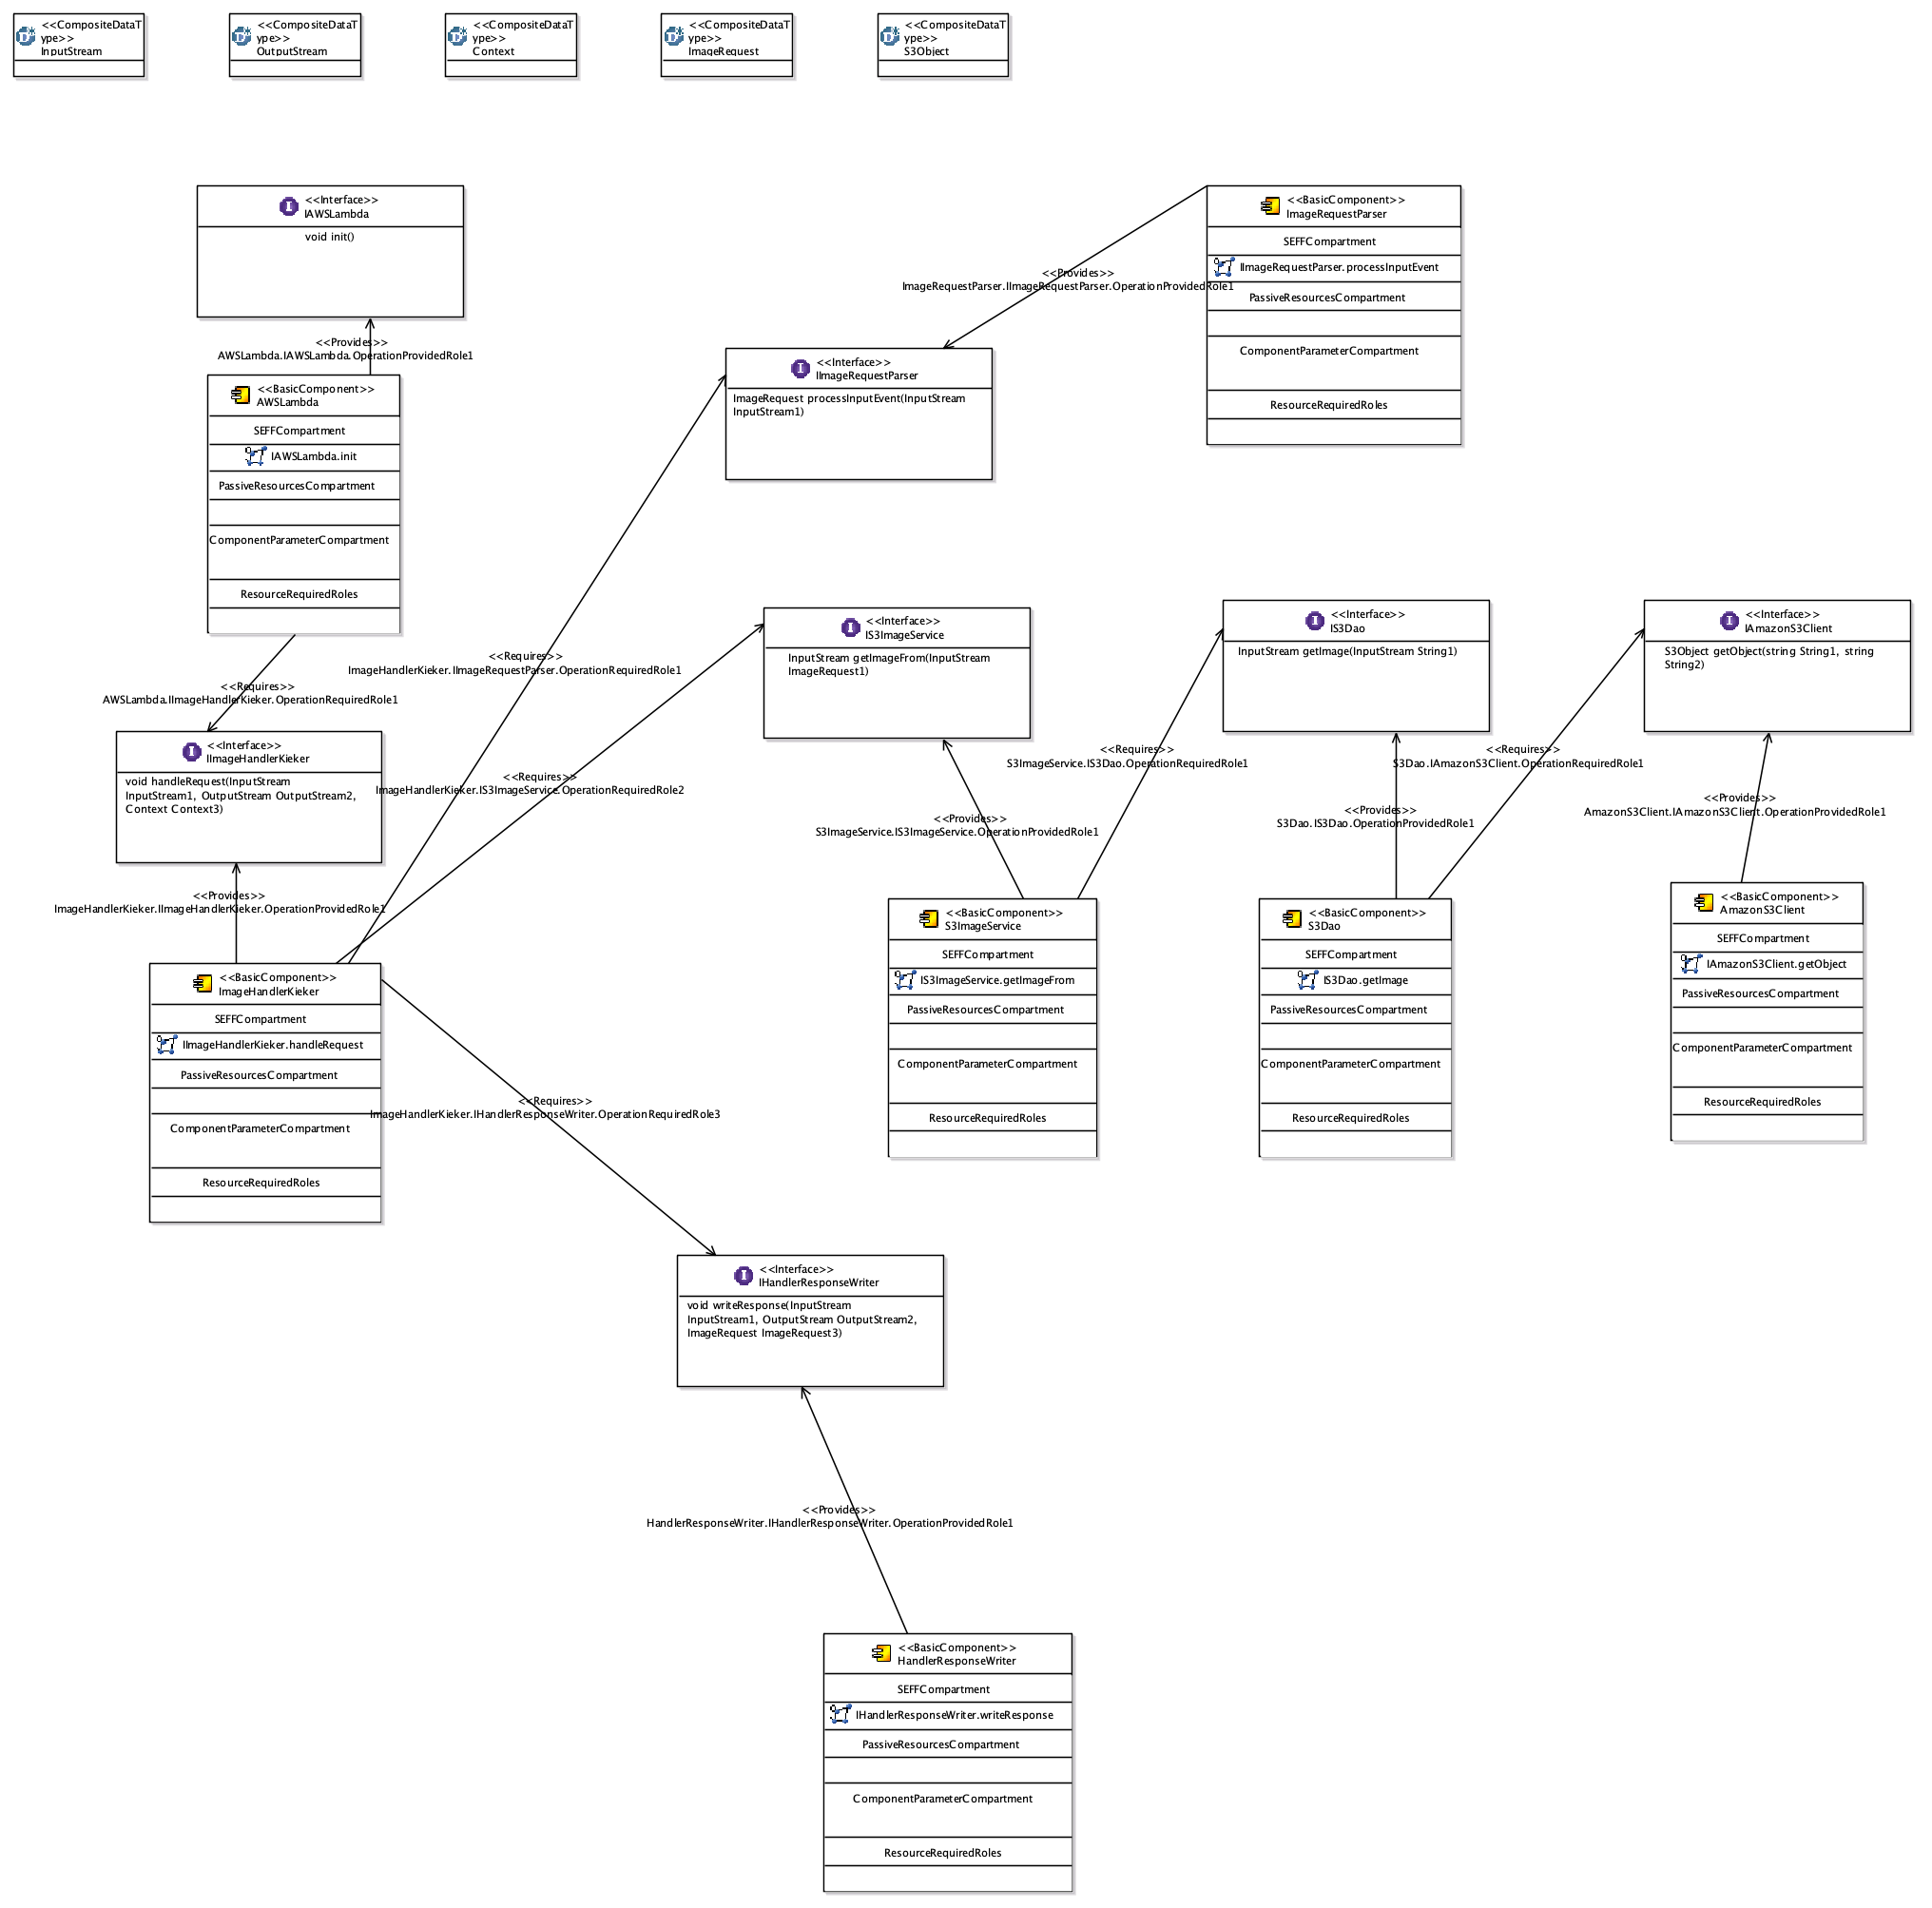
\includegraphics[width=20cm]{image-handler-extracted-repository-diagram.png}
  \caption{\emph{Image-Handler} publicando eventos de rendimiento al servicio AWS X-Ray}
  \label{fig:image-handler-pcm-model}
\end{figure}
\end{landscape}

%%%%%%%%%%%%%% Experimento 2

\subsection{Ejecución Secuencial Ininterrumpida de solicitudes de redimensionamiento}\label{sec:experimento-2}

En el experimento de la Sección \ref{sec:experimento-1} se realizaron múltiples solicitudes de redimensionamiento con el fin de extraer y crear un modelo de rendimiento, ejecutar simulaciones sobre este modelo y comparar los resultados con lo observado en una versión de \emph{Image Handler} real.

Una de las principales inquietudes durante la ejecución de funciones en la nube es determinar si la velocidad en la que se procesa una solicitud resulta ser baja y muestra una tendencia predecible. Los desarrolladores e implementadores necesitan evaluar esto para afinar el código fuente y la arquitectura para evitar cobros elevados por el uso de la plataforma.
De acuerdo con \cite{8360324}, una función puede pasar por dos grandes estados: uno ``fría'' y una ``caliente''. En el estado frío, la plataforma que soporta la función en la nube debe aprovisionar los recursos necesarios para ejecutar la función. Durante esta fase se pueden experimentar los tiempos de respuesta más prolongados. La fase caliente se da luego de que la plataforma que soporta la función reconoce que la función está siendo invocada constantemente y que, debido a este uso, necesita proporcionarle mayores recursos computacionales para brindar mejores tiempos de respuesta. Se espera que, en una función que se esté invocando constantemente, solamente un porcentaje muy bajo del tiempo se encuentre en estado frío y la mayor parte (mientras continúe siendo invocada) estará en estado caliente.


\subsubsection{Ejecución de solicitudes de redimensionamiento simultáneas para imágenes de tamaño menor a 500Kb}

%pic-14.jpeg (500Kb) 8:40 -> 9:05
%pic-27.jpeg (500Kb - 1Mb) 10:45 -> 1am
%pic-175.jpeg (1Mb - 2Mb) 2:16min

Para la realización de este experimento se contó con la siguiente configuración:
\begin{itemize}
    \item \emph{Sujeto de prueba:} La función Lambda IM-Simple
    \item \emph{Repositorio de imágenes:} \emph{Cluster} de 1000 imágenes de tamaño menor o igual a 500Kb alojadas en Amazon S3.
    \item \emph{Carga de trabajo:} 
    \begin{enumerate}
        \item 1000 invocaciones secuenciales de redimensionamiento de imágenes con dimensiones aleatorias a IM-Simple.
        \item 1000 invocaciones secuenciales de redimensionamient de una sola imagen a IM-Simple.
    \end{enumerate}
    \item \emph{Herramientas de medición:} Amazon Cloudwatch.
\end{itemize}

En la carga de trabajo \#1, utilizando imágenes aleatorias, la ejecución de las 1000 solicitudes de redimensionamiento fueron las mismas utilizadas para el experimento de la Sección \ref{sec:experimento-1}. 

La ejecución de las 1000 solicitudes de redimensionamiento tomó 2 horas y 36 minutos. Para la carga de trabajo \#2, utilizando una sola imagen, las 1000 solicitudes de redimensionamiento tomaron 25 minutos. Se modificó el \emph{script} en \texttt{Bash} del experimento de la Sección \ref{sec:experimento-1} para elegir aleatoriamente una imagen del \emph{cluster} de 1000 y generar 1000 solicitudes secuenciales a partir de esta con dimensiones de ancho y alto estáticas.

\begin{figure}[h]
\hspace{-1.0cm}
\begin{tikzpicture}
\begin{axis}[
    width=16cm, height=12cm,
    title={\small \textbf{1000 solicitudes de redimensionamiento en imágenes $\leq 500Kb$}},
    xlabel={\small Invocaciones a IM-Simple},
    ylabel={\small Tiempo (en $ms$)},
    xmin=-10, 
    xmax=1005,
    ymin=0, 
%    ymax=4100,
    %extra y ticks = {0.9,0.95},
    extra x tick style={tick label style={font=\footnotesize}},
    grid=major,
    grid style=dashed,
]

\addplot[mark=none,blue,smooth] table [col sep=comma] {datos/tiempos-de-respuesta-hasta-500kb-simple-2.csv};

\addplot[mark=none,red,smooth] table [col sep=comma] {datos/tiempos-de-respuesta-hasta-500kb-simple-una-imagen.csv};

\legend{\small Imágenes aleatorias, \small Imagen única} 
 
\end{axis}
\end{tikzpicture}
% Formato del caption para el índice de figuras %
\caption[hola]{1000 solicitudes de redimensionamiento en imágenes $\leq 500Kb$. La línea azul representa las solicitudes hechas utilizando imágenes aleatorias. La línea roja, las solicitudes utilizando una única imagen.}
\label{fig:1000-ejecuciones-secuenciales-500kb}
\end{figure}

En la figura \ref{fig:1000-ejecuciones-secuenciales-500kb} se muestran 1000 ejecuciones secuenciales utilizando imágenes aleatorias (línea azul) y utilizando una sola imagen (línea roja). La imagen de la línea roja es de tamaño 40Kb. Los resultados de los tiempos de respuesta muestran una tendencia marcada: la primera solicitud tomó mucho más tiempo que el resto. Una vez realizada la primera solicitud, los tiempos de respuesta de la función mejoraron considerablemente y no se observaron en las subsecuentes invocaciones tiempos de respuesta que llegaran a ser similares al primero. 


\subsubsection{Ejecución de solicitudes de redimensionamiento simultáneas para imágenes de tamaño mayor a 500Kb y menor o igual a 1Mb}

Para la realización de este experimento se contó con la siguiente configuración:
\begin{itemize}
    \item \emph{Sujeto de prueba:} La función Lambda IM-Simple
    \item \emph{Repositorio de imágenes:} \emph{Cluster} de 1000 imágenes de tamaño mayor a 500Kb y menor o igual a 1Mb alojadas en Amazon S3.
    \item \emph{Carga de trabajo:} 
    \begin{enumerate}
        \item 1000 invocaciones secuenciales de redimensionamiento de imágenes con dimensiones aleatorias a IM-Simple.
        \item 1000 invocaciones secuenciales de redimensionamient de una sola imagen a IM-Simple.
    \end{enumerate}
    \item \emph{Herramientas de medición:} Amazon Cloudwatch.
\end{itemize}

En la carga de trabajo \#1, utilizando imágenes aleatorias, la ejecución de las 1000 solicitudes de redimensionamiento fueron las mismas utilizadas para el experimento de la Sección \ref{sec:experimento-1}. 

La ejecución de las 1000 solicitudes de redimensionamiento tomó 2 horas y 36 minutos. Para la carga de trabajo \#2, utilizando una sola imagen, las 1000 solicitudes de redimensionamiento tomaron 2 horas y 30 minutos. Se modificó el \emph{script} en \texttt{Bash} del experimento de la Sección \ref{sec:experimento-1} para elegir aleatoriamente una imagen del \emph{cluster} de 1000 y generar 1000 solicitudes secuenciales a partir de esta con dimensiones de ancho y alto estáticas.

\begin{figure}[h]
\hspace{-1.5cm}
\begin{tikzpicture}
\begin{axis}[
    width=16cm, height=12cm,
    title={\small \textbf{1000 solicitudes de redimensionamiento en imágenes $500Kb \leq x \leq 1Mb$}},
    xlabel={\small Invocaciones a IM-Simple},
    ylabel={\small Tiempo (en $ms$)},
    xmin=-10, 
    xmax=1005,
    ymin=0, 
    extra x tick style={tick label style={font=\footnotesize}},
    grid=major,
    grid style=dashed,
]

\addplot[mark=none,blue,smooth] table [col sep=comma] {datos/tiempos-de-respuesta-hasta-1mb-simple-2.csv};

\addplot[mark=none,red,smooth] table [col sep=comma] {datos/tiempos-de-respuesta-hasta-1mb-simple-una-imagen.csv};
 
\legend{\small Imágenes aleatorias, \small Imagen única} 

\end{axis}
\end{tikzpicture}
\caption{1000 solicitudes de redimensionamiento en imágenes $500Kb \leq x \leq 1Mb$. La línea azul representa las solicitudes hechas utilizando imágenes aleatorias. La línea roja, las solicitudes utilizando una única imagen.}
\label{fig:1000-ejecuciones-secuenciales-1mb}
\end{figure}

En la figura \ref{fig:1000-ejecuciones-secuenciales-1mb} se muestran 1000 ejecuciones secuenciales utilizando imágenes aleatorias (línea azul) y utilizando una sola imagen (línea roja). La imagen de la línea roja es de tamaño 750Kb. Los resultados de los tiempos de respuesta muestran una tendencia marcada: la primer solicitud tomó mucho más tiempo que el resto. Una vez realizada la primer solicitud, los tiempos de respuesta de la función mejoraron considerablemente y, en el caso de las solicitudes de redimensionamiento en imágenes aleatorias, sí se logró observar un caso en el que el tiempo de respuesta fue similar al observado en la primera solicitud. En el caso de la imagen única no se observaron tiempos de respuesta que llegaran a ser similares al primero en posteriores invocaciones. 


\subsubsection{Ejecución de invocaciones de redimensionamiento simultáneas para imágenes de tamaño mayor a 1Mb y menor o igual a 2Mb}

Para la realización de este experimento se contó con la siguiente configuración:
\begin{itemize}
    \item \emph{Sujeto de prueba:} La función Lambda IM-Simple
    \item \emph{Repositorio de imágenes:} \emph{Cluster} de 1000 imágenes de tamaño mayor a 1Mb y menor o igual a 2Mb alojadas en Amazon S3.
    \item \emph{Carga de trabajo:} 
    \begin{enumerate}
        \item 1000 invocaciones secuenciales de redimensionamiento de imágenes con dimensiones aleatorias a IM-Simple.
        \item 1000 invocaciones secuenciales de redimensionamiento de una sola imagen a IM-Simple.
    \end{enumerate}
    \item \emph{Herramientas de medición:} Amazon Cloudwatch.
\end{itemize}

En la carga de trabajo \#1, utilizando imágenes aleatorias, la ejecución de las 1000 solicitudes de redimensionamiento fueron las mismas utilizadas para el experimento de la Sección \ref{sec:experimento-1}. 

La ejecución de las 1000 solicitudes de redimensionamiento tomó 2 horas y 36 minutos. Para la carga de trabajo \#2, utilizando una sola imagen, las 1000 solicitudes de redimensionamiento tomaron 2 horas y 16 minutos. Se modificó el \emph{script} en \texttt{Bash} del experimento de la Sección \ref{sec:experimento-1} para elegir aleatoriamente una imagen del \emph{cluster} de 1000 y generar 1000 solicitudes secuenciales a partir de esta con dimensiones de ancho y alto estáticas.


\begin{figure}[h]
\hspace{-1.5cm}
\begin{tikzpicture}
\begin{axis}[
    width=16cm, height=12cm,
    title={\small \textbf{1000 solicitudes de redimensionamiento en imágenes $1Mb \leq x \leq 2Mb$}},
    xlabel={\small Invocaciones a IM-Simple},
    ylabel={\small Tiempo (en $ms$)},
    xmin=-10, 
    xmax=1005,
    ymin=0, 
%    ymax=4100,
    %extra y ticks = {0.9,0.95},
    extra x tick style={tick label style={font=\footnotesize}},
    grid=major,
    grid style=dashed,
]

\addplot[mark=none,blue,smooth] table [col sep=comma] {datos/tiempos-de-respuesta-mas-de-1mb-simple-2.csv};

\addplot[mark=none,red,smooth, style={ultra thick}] table [col sep=comma] {datos/tiempos-de-respuesta-mas-de-1mb-simple-una-imagen.csv};

\legend{\small Imágenes aleatorias, \small Imagen única} 
 
\end{axis}
\end{tikzpicture}
\caption{1000 solicitudes de redimensionamiento en imágenes $1Mb \leq x \leq 2Mb$. La línea azul representa las solicitudes hechas utilizando imágenes aleatorias. La línea roja, las solicitudes utilizando una única imagen.}
\label{fig:1000-ejecuciones-secuenciales-2mb}
\end{figure}

En la figura \ref{fig:1000-ejecuciones-secuenciales-2mb} se muestran 1000 ejecuciones secuenciales utilizando imágenes aleatorias (línea azul) y utilizando una sola imagen (línea roja). La imagen de la línea roja es de tamaño 1,4Mb. Los resultados de los tiempos de respuesta muestran una tendencia similar a los casos anteriores: la primer solicitud tomó mucho más tiempo que el resto. Una vez realizada la primer solicitud, los tiempos de respuesta de la función mejoraron considerablemente y, en el caso de las solicitudes de redimensionamiento en imágenes aleatorias, sí se logró observar un caso en el que el tiempo de respuesta fue similar al observado en la primera solicitud. En el caso de la imagen única no se observaron tiempos de respuesta que llegaran a ser similares al primero en posteriores invocaciones. 

\subsubsection{Análisis de resultados}
Luego de las invocaciones de redimensionamiento tanto en imágenes aleatorias como en una sola imagen, se pudo observar que, si bien en las primeras invocaciones se experimenta mayores tiempos de respuesta, los tiempos de respuesta entregados por la función Lambda lograron bajar significativamente y en los casos de las invocaciones de redimiensionamiento en una sola imagen, estos tiempos lograron mantenerse sumamente estables.

Este comportamiento sugiere que en la invocación de una función Lambda en AWS, la plataforma subyacente primero necesita aplicar tareas de aprovisionamiento para poner a disposición la función y, una vez que esto se realiza, la función paulatinamente va pasando a un estado ``caliente'' conforme van arribando las invocaciones de redimensionamiento. Aunque la arquitectura del servicio AWS Lambda no se encuentra disponible públicamente, en árticulos en Internet y en proyectos paralelos como SAM Cli y \emph{AWS Lambda container image converter tool}\footnote{\url{https://github.com/awslabs/aws-lambda-container-image-converter}} se sugiere el uso de contenedores Docker que son provisionados con el código de la función y que se encargan de procesar las invocaciones entrantes. 

\paragraph{Relación con el modelo de rendimiento obtenido} El modelo de rendimiento obtenido y las simulaciones hechas son agnósticos a los estados ``frío'' o ``caliente'' que se muestran en las observaciones. El principal objetivo de los simuladores de PCM es el de obtener múltiples combinaciones de ejecuciones de una arquitectura de software dada y, a menos que un comportamiento o característica de esta logre ser introducido en el modelo es que su impacto debería de verse reflejado en las simulaciones.

Si bien en el modelo obtenido no se introdujo esto explícitamente, las mediciones muestran que los tiempos de respuesta más prolongados se corresponden con el momento en que la función estaba en estado ``frío'', por ejemplo, durantes las primeras invocaciones. Si se toma como referencia el primer experimento ejecutado en la Sección \ref{sec:experimento-1}, invocaciones de redimensionamiento en imágenes menores o iguales a 500Kb, en la figura \ref{fig:comparacion-imsimple-palladio-500kb}, la primera medición a IM-Simple dió como resultado 4.1s y las subsecuentes 999 invocaciones bajaron a 1,6 segundos o menos; muchas de ellas incluso fueron menores a medio segundo. En los resultados de este experimento, existe un 95\% de probablidades que los tiempos de respuesta de las invocaciones sean de 1,6 segundos o menos, lo que, visto desde otro ángulo, quiere decir que existe un 5\% de probabilidad que los tiempos de respuesta de las  invocaciones tomen entre 1,6 y 4 segundos en ser procesadas. Ahora bien, aunque 5\% parece ser una probabilidad muy alta y que no refleja lo visto en las mediciones, cuando se vuelve a los resultados de las simulaciones se observa que hay probabilidad mayor al 99\% de que una invocación de redimensionamiento tenga un tiempo de respuesta igual o menor a 2 segundos. Esto quiere decir que hay una probabilidad de menos del 1\% de que una invocación a la función Lambda tome entre 2 y 4 segundos en ser procesada. En el caso de las simulaciones de la Figura \ref{fig:comparacion-imsimple-palladio-500kb} solamente 6 casos muestran tiempos de respuesta de entre 2 y 4 segundos lo que representa un 0.006\% del total de las simulaciones realizadas.

Lo anterior señala que, para el caso de \emph{Image Handler}, las simulaciones con los tiempos de respuesta más prolongados representan una cantidad muy pequeña de la totalidad de los casos y que, estos casos se pueden interpretar como potenciales escenarios de la función Lambda en estado frío. Las simulaciones muestran que a pesar del impacto que tienen estos escenarios en las invocaciones, estos realmente no llegan afectar el comportamiento general de la función Lambda. 

Con respecto a los resultados de este experimento y su relación con los escenarios de invocaciones de redimiensionamiento en imágenes de tamaño de 500Kb y menor o igual a 1Mb, e imágenes de tamaño de 1Mb y menor a 2Mb, expuestas en la Sección \ref{sec:experimento-1}, se puede emplear un análisis similar: las simulaciones que reportan los tiempos de respuesta más prolongados tienen el potencial de caracterizar las ejecuciones de la función en estado ``frío''.

%%%%%%%%%%%%%% Experimento 3
\subsection{Variación del intervalo de las invocaciones de redimensionamiento}\label{sec:experimento-3}

Este experimento se plantea como una variante del expuesto en la Sección \ref{sec:experimento-2}, donde se evaluaba el efecto de las invocaciones simultáneas a la función Lambda. Acá se plantea variar el intervalo entre invocaciones a la función Lambda con el fin de valorar los efectos en el comportamiento de la función y si el modelo obtenido en la Sección \ref{sec:experimento-1} contribuye a explicar algo de lo observado; en particular si los intervalos entre las invocaciones hacen que el rendimiento de la función se considere ``fría'' o ``caliente'' en algún punto.

\subsubsection{Estrategia de intervalo de invocaciones a \emph{Image Handler}}
Para evaluar los efectos de los intervalos de lanzamiento en las invocaciones a \emph{Image Handler}, se propone la ejecución de un número de invocaciones secuencial (una ráfaga), luego entrar en un tiempo de espera y luego, aplicar otra ráfaga de invocaciones. 

El tiempo de espera entre ráfagas se irá incrementando al doble del tiempo de espera anterior. Por ejemplo, si el primer tiempo de espera es de 2 minutos, el siguiente será de 4 minutos, luego 8, 16, 32 minutos y así sucesivamente. Para este experimento se propone utilizar un tiempo de espera inicial de 10 minutos, para luego aumentarlo en subsecuentes ráfagas de invocaciones.

\subsubsection{Ejecución de ráfagas de invocaciones de redimensionamiento para imágenes de tamaño menor a 500Kb}

Para la realización de este experimento se utilizó la siguiente configuración base:
\begin{itemize}
    \item \emph{Sujeto de prueba:} La función Lambda IM-XRay.
    \item \emph{Repositorio de imágenes:} \emph{Cluster} de 1000 imágenes de tamaño menor o igual a 500Kb alojadas en Amazon S3.
    \item \emph{Carga de trabajo:} 100 invocaciones secuenciales de redimensionamiento de imágenes con dimensiones aleatorias a IM-XRay seguido de un tiempo de espera de 10, 20 y 40 minutos.      
    \item \emph{Herramientas de medición:} Amazon Cloudwatch y Amazon X-Ray.
\end{itemize}
 
De acuerdo con lo observado en los experimentos anteriores, luego de la primera invocación, las subsiguientes hacen que la función entre en un estado ``caliente''. Por esta razón, ejercitar la función con una ráfaga de 100 invocaciones haría que se logre llegar a este estado fácilmente.

A diferencia de los experimentos anteriores, se utiliza la versión de IM-XRay en lugar de IM-Simple. La razón es que se quiere sacar provecho a las herramientas de monitoreo de AWS X-Ray para determinar si la función pasa de un estado \emph{frío $\rightarrow$ caliente $\rightarrow$ frío} y determinar el impacto de este cambio en el tiempo de respuesta.

\subsubsection{Variando el intervalo de las invocaciones de redimensionamiento en imágenes $\leq 500Kb$}\label{sec:rafagas-hasta-500kb}

La Figura \ref{fig:rafagas-hasta-500kb} muestra 400 invocaciones de redimensionamiento en imágenes menores a 500Kb divididas en 100 ráfagas cada una. En la primer ráfaga la función se encuentra en estado ``frío'', sucede el aprovisionamiento inicial. Luego de esta primer invocación la función va entrando paulatinamente en estado ``caliente'' y se logra observar que para la mayoría de los casos las invocaciones de redimensionamiento no llegan a tomar más de 1,5 segundos. El tiempo promedio de ejecución de una ráfaga fue de 2 minutos y 45 segundos.

\begin{figure}
\hspace{-1.0cm}
\begin{tikzpicture}
\begin{axis}[
    width=16cm, height=12cm,
    title={\small \textbf{4 ráfagas de 100 invocaciones de redimensionamiento en imágenes $\leq 500Kb$}},
    xlabel={\small Invocaciones a IM-XRay},
    ylabel={\small Tiempo (en $ms$)},
    xmin=-10, 
    xmax=535,
    ymin=0, 
%    ymax=6000,
%    extra x ticks = {90,165},
    extra x tick style={tick label style={font=\footnotesize}},
    grid=major,
    grid style=dashed,
]

\addplot[mark=none,blue,smooth] table [col sep=comma] {datos/hasta-500kb-rafagas-bck-1.csv};
\addplot[color=red, mark=none, dashed, opacity=0.5] coordinates {(103,0)(103,10000)(117,10000)(117,0)};
\addplot[mark=none,blue,smooth] table [col sep=comma] {datos/hasta-500kb-rafagas-bck-2.csv};
\addplot[color=red, mark=none, dashed, opacity=0.5] coordinates {(223,0)(223,10000)(257,10000)(257,0)};
\addplot[mark=none,blue,smooth] table [col sep=comma] {datos/hasta-500kb-rafagas-bck-3.csv};
\addplot[color=red, mark=none, dashed, opacity=0.5] coordinates {(362,0)(363,10000)(429,10000)(429,0)};
\addplot[mark=none,blue,smooth] table [col sep=comma] {datos/hasta-500kb-rafagas-bck-4.csv};

%\legend{\small Imágenes aleatorias, \small Imagen única} 
 
\end{axis}
\end{tikzpicture}
\caption{El espacio delimitado por la línea punteada roja representa 10 minutos de inactividad entre la primer ráfaga y la segunda. El segundo espacio delimitado por la línea punteada roja representa 20 minutos de inactividad entre la segunda y la tercera ráfaga.}
\label{fig:rafagas-hasta-500kb}
\end{figure}

En la segunda ráfaga, luego de 10 minutos, la función no experimenta un tiempo de respuesta inicial similar al de la primer ráfaga. Esto quiere decir que pasados 10 minutos de inactividad entre la primera y segunda ráfagas, la función continúa en estado caliente.

En la tercera ráfaga, luego de 20 minutos de haberse ejecutado la última invocación de redimensionamiento de la ráfaga anterior, sí se llega observar un tiempo de respuesta inicial alto. AWS X-Ray reporta que en esta invocación inicial se tuvo que re-aprovisionar la función, lo que sugiere que, durante los 20 minutos de inactividad entre una ráfaga y otra, la función fue pasando progresivamente a un estado ``frío'' debido a que la plataforma pudo determinar que el nivel de actividad de la función (cantidad de invocaciones) fue decreciendo hasta un punto en donde no detectó actividad alguna.

La última ráfaga también experimentó un tiempo de respuesta inicial alto. Esta vez un poco mayor al de la ráfaga anterior pero menor a la de la primer ráfaga. Hubo 40 minutos de inactividad entre la tercera ráfaga y la cuarta. 

\subsubsection{Variando el intervalo de las invocaciones de redimensionamiento en imágenes $500Kb \leq x \leq 1Mb$}

Se hizo el mismo ejercicio que en la Sección \ref{sec:rafagas-hasta-500kb}. La Figura \ref{fig:rafagas-hasta-1mb} muestra los resultados de la ejecución de 5 ráfagas de 100 invocaciones cada una. El tiempo promedio de ejecución de una ráfaga fue de 9 minutos y 15 segundos. En la primera invocación de la primer ráfaga se obtuvo un tiempo de respuesta alto (función en estado frío). En la segunda ráfaga no se observó tiempos de respuesta elevados debido a que la función se encontraba en estado ``caliente''. 

\begin{figure}
\hspace{-1cm}
\begin{tikzpicture}
\begin{axis}[
    width=16cm, height=12cm,
    title={\small \textbf{5 ráfagas de 100 invocaciones de redimensionamiento en imágenes $500Kb \leq x \leq 1Mb$}},
    xlabel={\small Invocaciones a IM-XRay},
    ylabel={\small Tiempo (en $ms$)},
    xmin=-10, 
    xmax=775,
    ymin=0, 
    ymax=14000,
%    extra x ticks = {90,165},
    extra x tick style={tick label style={font=\footnotesize}},
    grid=major,
    grid style=dashed,
]

\addplot[mark=none,blue,smooth] table [col sep=comma] {datos/hasta-1mb-rafagas-1.csv};
\addplot[color=red, mark=none, dashed, opacity=0.5] coordinates {(103,0)(103,10000)(117,10000)(117,0)};
\addplot[mark=none,blue,smooth] table [col sep=comma] {datos/hasta-1mb-rafagas-2.csv};
\addplot[color=red, mark=none, dashed, opacity=0.5] coordinates {(223,0)(223,10000)(257,10000)(257,0)};
\addplot[mark=none,blue,smooth] table [col sep=comma] {datos/hasta-1mb-rafagas-3.csv};
\addplot[color=black, mark=none, dashed, style={ultra thick}] coordinates {(260,8082)(260,14000)};
\addplot[color=red, mark=none, dashed, opacity=0.5] coordinates {(362,0)(363,10000)(429,10000)(429,0)};
\addplot[mark=none,blue,smooth] table [col sep=comma] {datos/hasta-1mb-rafagas-4.csv};
\addplot[color=black, mark=none, dashed, style={ultra thick}] coordinates {(434,9356)(434,14000)};
\addplot[color=red, mark=none, dashed, opacity=0.5] coordinates {(535,0)(535,10000)(671,10000)(671,0)};
\addplot[mark=none,blue,smooth] table [col sep=comma] {datos/hasta-1mb-rafagas-5.csv};
 
\end{axis}
\end{tikzpicture}
\caption{El espacio delimitado por la línea punteada roja representa 10 minutos de inactividad entre la primer ráfaga y la segunda. El espacio delimitado por la línea punteada verde representa 20 minutos de inactividad entre la segunda y la tercera ráfaga.}
\label{fig:rafagas-hasta-1mb}
\end{figure}

En la primera invocación de la tercera y cuarta ráfaga, AWS X-Ray reportó que en ambas hubo que re-aprovisionar la función. Es decir, el tiempo de inactividad entre la segunda ráfaga (20 minutos) y entre la tercera y la cuarta (40 minutos) fue suficiente para que la plataforma volviera a marcar la función como fría de nuevo. Lo interesante de estas dos primeras invocaciones, es que, a pesar que la plataforma tuvo que volver a re-aprovisionar la función, los tiempos de respuesta reportados fueron mucho más bajos que el de la invocación inicial de la primer ráfaga. En la Tabla \ref{table:rafagas-hasta-1mb-tiempos-primera-invocacion} se pueden ver los tiempos de respuesta de las primeras invocaciones de cada ráfaga.

\begin{table}
    \centering
    \begin{tabular}{l|r}
        \toprule[1.5pt]
        \multicolumn{2}{c}{\textbf{Entre 500Kb a 1Mb}} \\
        \midrule
        Ráfaga  & Tiempo de 1º invocación \\
        \midrule
        \#1  & 13s \\
        \#2  & N.A. \\        
        \#3  & 8s \\        
        \#4  & 9s \\        
        \#5  & 11s \\                                
        \bottomrule[1.5pt]
    \end{tabular}
    \caption{Tiempo de respuesta de la primer invocación de redimensionamiento en cada ráfaga.}
    \label{table:rafagas-hasta-1mb-tiempos-primera-invocacion}
\end{table}

En la quinta ráfaga, el tiempo de respuesta de la primera invocación se elevó de nuevo. El tiempo de inactividad entre la cuarta ráfaga y la quinta fue de 80 minutos. 

Debido a que los tiempos iniciales de la tercera y cuarta ráfaga fueron bajos (aunque AWS X-Ray reporta que para cada uno de ellos fue necesaria re-aprovisionar la función), fue que se la ejecución de una quinta ráfaga se hizo necesaria con el fin de validar que, conforme los tiempos de inactividad entre ráfagas aumenta, el tiempo de respuesta de la primera invocación también aumenta. 

\subsubsection{Variando el intervalo de las invocaciones de redimensionamiento en imágenes $1Mb \leq x \leq 2Mb$}

Para este caso, el tiempo promedio de ejecución de una ráfaga fue de 13 minutos y 15 segundos. En la ejecución de cada ráfaga, AWS X-Ray reportó que fue necesario re-aprovisionar la función cuando se ejecutó la primera invocación de cada ráfaga. En la Figura \ref{fig:rafagas-hasta-2mb} se muestran los resultados de la ejecución de las cuatro ráfagas.

\begin{figure}
\hspace{-1.5cm}
\begin{tikzpicture}
\begin{axis}[
    width=16cm, height=12cm,
    title={\small \textbf{4 ráfagas de 100 invocaciones de redimensionamiento en imágenes $1Mb \leq x \leq 2Mb$}},
    xlabel={\small Invocaciones a IM-XRay},
    ylabel={\small Tiempo (en $ms$)},
    xmin=-10, 
    xmax=535,
    ymin=0, 
    ymax=16000,
%    extra x ticks = {90,165},
    extra x tick style={tick label style={font=\footnotesize}},
    grid=major,
    grid style=dashed,
]

\addplot[mark=none,blue,smooth] table [col sep=comma] {datos/hasta-2mb-rafagas-1.csv};
\addplot[color=red, mark=none, dashed, opacity=0.5] coordinates {(103,0)(103,10000)(117,10000)(117,0)};
\addplot[mark=none,blue,smooth] table [col sep=comma] {datos/hasta-2mb-rafagas-2.csv};
\addplot[color=red, mark=none, dashed, opacity=0.5] coordinates {(223,0)(223,10000)(257,10000)(257,0)};
\addplot[mark=none,blue,smooth] table [col sep=comma] {datos/hasta-2mb-rafagas-3.csv};
\addplot[color=red, mark=none, dashed, opacity=0.5] coordinates {(362,0)(363,10000)(429,10000)(429,0)};
\addplot[mark=none,blue,smooth] table [col sep=comma] {datos/hasta-2mb-rafagas-4.csv};
 
\end{axis}
\end{tikzpicture}
\caption{El espacio delimitado por la línea punteada roja representa 10 minutos de inactividad entre la primer ráfaga y la segunda. El espacio delimitado por la línea punteada verde representa 20 minutos de inactividad entre la segunda y la tercera ráfaga.}
\label{fig:rafagas-hasta-2mb}
\end{figure}

Los tiempos de respuesta de las primeras invocaciones de cada ráfaga resultaron ser más similares entre sí y, también se pudo observar que cuando existen tiempos de inactivad más prolongados, como el que entre la ráfaga tres y la cuando que es de 40 minutos, a la siguiente invocación le toma un mayor tiempo de respuesta que la primer invocación de la ráfaga anterior.

\subsubsection{Análisis de resultados}
La principal observación que arrojó este experimento es que conforme van aumentando los tiempos de inactividad en la función Lambda, también van aumentando los tiempos de respuesta entregados por la primera invocación luego de este tiempo de inactividad. 

De acuerdo con \cite{cold-starts-aws-lambda-1}, una vez que una función ha sido instalada en la plataforma, la primera invocación debe pasar por el proceso de aprovisionamiento. Luego de que esta primer invocación es procesada, la función pasa a un estado activo o ``caliente'' y el contenedor que la soporta se puede reutilizar para subsecuentes invocaciones. Cuando se detecta que la función se vuelve inactiva o ``fría'', el contenedor que la soporta se vuelve candidato a ser ``reciclado'' para ser utilizado por otra función que lo necesite.

Si bien no hay un tiempo límite definido para decidir cuándo el contenedor va a ser reciclado o no, los resultados de este experimento y los expuestos en \cite{cold-starts-aws-lambda-1} y \cite{cold-starts-aws-lambda-2} demuestran que entre mayor sean los tiempos de inactividad de una función, mayor será la probabilidad de que el contenedor que la soporta sea reciclado y que, cuando se vuelva a invocar a la función, se experimente un tiempo de respuesta mayor al promedio debido al proceso de aprovisionamiento. 

Según las mediciones en \cite{cold-starts-aws-lambda-1}, el tiempo de vida de un contenedor no parece darse en forma determinística pero se estima que está entre los 25 a 65 minutos. Una contenedor inactivo casi siempre se mantiene vivo por 25 minutos, luego de eso la probabilidad de que sea desechado crece lentamente y llega a alcanzar el 100\% luego de alrededor de 1 hora luego de la última invocación.

\paragraph{Relación con el modelo de rendimiento obtenido} En el experimento de la Sección \ref{sec:experimento-1} se obtuvo un modelo de rendimiento a partir una sola ráfaga invocaciones secuenciales de redimensionamiento. No se introdujo tiempos de inactividad. 

Aquí, aunque se introducen tiempos de inactividad entre ráfagas, se presenta una tendencia que se ha repetido a lo largo de los tres experimentos ejecutados hasta este momento: las primeras invocaciones reportan mayores tiempos de respuesta, especialmente la primera invocación, y conforme la función va recibiendo más y más invocaciones, su tiempo de respuesta tiende a bajar considerablemente. Esta es una característica que el modelo obtenido logró reconocer y, de igual manera como en los experimentos anteriores, las invocaciones en donde los tiempos de respuesta fueron mayores representan un porcentaje muy bajo ($\approx$ 1\%) del total de invocaciones en una ráfaga, por lo que cuando el modelo reporte invocaciones con tiempos de respuesta alto se puede afirmar para el caso de \emph{Image Handler} que estas invocaciones serán muy pocas y que probablemente representen momentos en donde la función tuvo que pasar forzozamente de un estado ``frío'' a uno ``caliente''.


En PCM, el comportamiento asociado a las invocaciones basadas en ráfagas y tiempos de inactividad podría llegar a ser introducido con un modelo de uso personalizado el cual pueda tomar en cuenta las particularidades del cómo es que una arquitectura de software puede ser potencialmente utilizada pero, la forma en la que PCM reporta los resultados de las simulaciones es la misma independientemente del modelo de uso (o de cualquier otro modelo) utilizado. Es por esto que, en términos de resultados, PCM siempre va a entregar resultados basados en la probabilidad de que una determinada simulación se ejecute en una arquitectura dada. Lo anterior se usa para aclarar que mientras se utilice PCM para ejecutar simulaciones mediante el esquema de ráfaga/tiempo de espera, los resultados obtenidos no vendrán dados de forma específica para cada ráfaga ejecutada, sino más bien serán presentados de forma general.

%%%%%%%%%%%%%% Experimento 4
\subsection{Comparación de \texttt{SAM CLI} con observaciones reales de AWS Lambda}\label{sec:experimento-4} 
\emph{Serverless Application Model} o \texttt{SAM CLI} es la primera herramienta desarrollada por Amazon para probar funciones Lambda localmente. \texttt{SAM CLI} permite desarrollar funciones Lambda en cualquiera de los lenguajes de programación soportados por el servicio AWS Lambda y probarlos sin necesidad de instalarlos directamente en el servicio. Para emular el servicio, \texttt{SAM CLI}, hace uso de Docker para instalar y ejecutar el código de una función en un contenedor especializado para tal fin. 

\texttt{SAM CLI} no es la primera herramienta desarrollada para probar, instalar y emular funciones Lambda en un entorno local, pero si es la primera desarrollada por Amazon por lo que se espera que mediante su uso se pueda tener una aproximación muy cercana del comportamiento que va a tener una función Lambda cuando esté en producción.

En este experimento se propone explorar el comportamiento de \emph{Image Handler} cuando se ejecutan invocaciones de redimensionamiento en \texttt{SAM CLI} y, comparar lo obtenido con invocaciones de redimensionamiento efectuadas en el servicio de AWS Lambda en producción. Los resultados de este experimento permitirán determinar si las invocaciones hechas en \texttt{SAM CLI} entregan tiempos de respuesta similares a los del servicio AWS Lambda para que, de esta forma se pueda considerar \texttt{SAM CLI} como una herramienta confiable para simulación de invocaciones de rendimiento.

\subsubsection{Estrategia de comparación de invocaciones de redimensionamiento en \texttt{SAM CLI} y AWS Lambda}

Similar a los experimentos anteriores, se propone ejecutar 1000 ejecuciones de redimensionamiento a \emph{Image Handler}. Para valorar la similitud entre los resultados, el conjuntos\ de invocaciones utilizadas serán las mismas para \texttt{SAM CLI} y AWS Lambda: la $k-$ésima invocación a \emph{Image Handler} realizada por medio de \texttt{SAM CLI} será igual a la $k-$ésima invocación realizada en AWS Lambda.

\subsubsection{Ejecución de 1000 invocaciones de redimensionamiento para imágenes de tamaño menor a 500Kb}

Para la realización de este experimento se utilizó la siguiente configuración base:
\begin{itemize}
    \item \emph{Sujeto de prueba:} La función lambda IM-Simple.
    \item \emph{Repositorio de imágenes:} \emph{Cluster} de 1000 imágenes de tamaño menor o igual a 500Kb.
    \item \emph{Carga de trabajo:} 1000 invocaciones secuenciales de redimensionamiento de imágenes en IM-Simple.
    \item \emph{Herramientas de medición:} Amazon Cloudwatch.
\end{itemize}

Configuración para la realización del experiento en \texttt{SAM CLI}:
\begin{itemize}
    \item \emph{Sujeto de prueba:} La función lambda IM-Simple.
    \item \emph{Ambiente:} \texttt{SAM CLI} instalado en máquina virtual alojada en el servicio AWS EC2\footnote{\url{https://aws.amazon.com/ec2/}}, de tipo \texttt{t2.large}\footnote{\url{https://aws.amazon.com/ec2/instance-types/t2/}}.
    \item \emph{Repositorio de imágenes:} \emph{Cluster} de 1000 imágenes de tamaño menor o igual a 500Kb.
    \item \emph{Carga de trabajo:} 1000 invocaciones secuenciales de redimensionamiento de imágenes en IM-Simple.
    \item \emph{Herramientas de medición:} Bitácoras de \texttt{SAM CLI}.
\end{itemize}


\begin{figure}
\hspace{-1cm}
\begin{tikzpicture}
	\begin{axis}[
	width=16cm, height=12cm, xmin=0, ymin=0,
	xmax=1010, 
%	ymax=14500,
	title={\textbf{\emph{Image Handler vs} \texttt{SAM CLI}: redimensionamiento en imágenes de tamaño $\leq 500Kb$}},
	xlabel={\small Número de ejecución de solicitud de redimensionamiento},
	ylabel={\small Milisegundos},
	grid=major, grid style=dashed, label style={font=\small},
	tick label style={font=\footnotesize},
	scatter/classes={%
		a={mark=square*,blue},%
		b={mark=square*,red},%
		c={mark=o,draw=black}}]			
	\addplot[scatter,only marks,%
		scatter src=explicit symbolic]%
	table[meta=label, col sep=comma] {datos/xy-sam-data-500kb.csv};
	\legend{Solicitudes a \emph{Image Handler}, Solicitudes en \texttt{SAM CLI}}
	\end{axis}
\end{tikzpicture}
\caption{Solicitudes de redimensionamiento de imágenes de tamaño $1Mb \leq x \leq 2Mb$}
\label{fig:comparacion-sam-500kb}
\end{figure}

\begin{table}
    \centering
    \begin{tabular}{l|r|r|r}
        \toprule[1.5pt]
         \multicolumn{4}{c}{\textbf{AWS Lambda vs SAM CLI: Hasta 500Kb}} \\
         \midrule
         & AWS Lambda & \texttt{SAM CLI} & Diferencia \\ 
         \midrule
        Duración & 15min & 90min & -- \\
        Tiempo promedio  & 571.15ms & 804.35ms & 233.20ms\\
        Desviación estándar & 449.76ms & 162.22ms & 287.54ms \\
        Varianza & 202281.41 & 26314.94 & -- \\
        Mediana & 698.28ms & 771.52ms & -- \\
        Coeficiente de variación & 0.64 & 0.21 & -- \\                        
        \bottomrule[1.5pt]
    \end{tabular}
    \caption{Resumen de datos estadísticos}
    \label{table:sam-datos-estadisticos-hasta-500kb}
\end{table}

\paragraph{Resultados:} La Figura \ref{fig:comparacion-sam-500kb}, muestra la comparación de los tiempos de respuesta de las 1000 invocaciones realizadas y en la tabla \ref{table:sam-datos-estadisticos-hasta-500kb} un resumen de los datos estadísticos obtenidos. A primera vista se puede ver que el conjunto de tiempos de respuesta de las invocaciones cuando se utilizó \texttt{SAM CLI} fue más homogéneo que las invocaciones en AWS Lambda. Esto también se refleja en los coeficientes de variación: 0.64 y 0.21 para las invocaciones en AWS Lambda y \texttt{SAM CLI} respectivamente, lo que claramente sugiere que el conjunto de tiempos de respuesta obtenido de las invocaciones de \texttt{SAM CLI} es más homogéneo que el de AWS Lambda. Esto también lo confirma una menor desviación estándar en el conjunto de tiempos de respuesta de las invocaciones hechas mediantes \texttt{SAM CLI}. 

En la tabla \ref{table:sam-datos-estadisticos-hasta-500kb}, el tiempo promedio de las invocaciones realizadas en AWS Lambda fue más bajo que el de \texttt{SAM CLI}. En \texttt{SAM CLI}, el menor tiempo de respuesta fue de 545.74ms mientras que en los resultados obtenidos de AWS Lambda aproximadamente el 56\% de los resultados estuvo por debajo de los 545.74ms. Esto indica que a pesar que el conjunto de los tiempos de respuesta de \texttt{SAM CLI} es más homogéneo, los tiempos obtenidos de AWS Lambda muestran un mejor rendimiento.

\subsubsection{Ejecución de 1000 invocaciones de redimensionamiento para imágenes de tamaño $500Kb \leq x \leq 1Mb$}

Para la realización de este experimento se utilizó la siguiente configuración base:
\begin{itemize}
    \item \emph{Sujeto de prueba:} La función lambda IM-Simple.
    \item \emph{Repositorio de imágenes:} \emph{Cluster} de 1000 imágenes de tamaño mayor a 500Kb y menor o igual a 1Mb.
    \item \emph{Carga de trabajo:} 1000 invocaciones secuenciales de redimensionamiento de imágenes en IM-Simple.
    \item \emph{Herramientas de medición:} Amazon Cloudwatch.
\end{itemize}

Configuración para la realización del experiento en \texttt{SAM CLI}:
\begin{itemize}
    \item \emph{Sujeto de prueba:} La función lambda IM-Simple.
    \item \emph{Ambiente:} \texttt{SAM CLI} instalado en máquina virtual alojada en el servicio AWS EC2, de tipo \texttt{t2.large}.
    \item \emph{Repositorio de imágenes:} \emph{Cluster} de 1000 imágenes de tamaño mayor o igual a 500Kb y menor a 1Mb.
    \item \emph{Carga de trabajo:} 1000 invocaciones secuenciales de redimensionamiento de imágenes en IM-Simple.
    \item \emph{Herramientas de medición:} Bitácoras de \texttt{SAM CLI}.
\end{itemize}

\begin{figure}
\hspace{-1cm}
\begin{tikzpicture}
	\begin{axis}[
	width=16cm, height=12cm, xmin=0, ymin=0,
	xmax=1010, 
%	ymax=14500,
	title={\textbf{\emph{Image Handler vs} \texttt{SAM CLI}: redimensionamiento en imágenes de tamaño $500Kb \leq x \leq 1Mb$}},
	xlabel={\small Número de ejecución de solicitud de redimensionamiento},
	ylabel={\small Milisegundos},
	grid=major, grid style=dashed, label style={font=\small},
	tick label style={font=\footnotesize},
	scatter/classes={%
		a={mark=square*,blue},%
		b={mark=square*,red},%
		c={mark=o,draw=black}}]			
	\addplot[scatter,only marks,%
		scatter src=explicit symbolic]%
	table[meta=label, col sep=comma] {datos/xy-sam-data-1mb.csv};
	\legend{Solicitudes a \emph{Image Handler}, Solicitudes en \texttt{SAM CLI}}
	\end{axis}
\end{tikzpicture}
\caption{Solicitudes de redimensionamiento de imágenes de tamaño $500kb \leq x \leq 1Mb$}
\label{fig:comparacion-sam-1mb}
\end{figure}

\begin{table}
    \centering
    \begin{tabular}{l|r|r|r}
        \toprule[1.5pt]
         \multicolumn{4}{c}{\textbf{AWS Lambda vs SAM CLI: Hasta 1Mb}} \\
         \midrule
         & AWS Lambda & \texttt{SAM CLI} & Diferencia \\ 
         \midrule
        Duración & 72min & 218min & -- \\
        Tiempo promedio  & 4345.80ms & 1969.49ms & 2376.31ms\\
        Desviación estándar & 1867.64ms & 524.95ms & 1342.69ms \\
        Varianza & 3488063 & 275569.63 & -- \\
        Mediana & 3898.82ms & 1851.99ms & -- \\
        Coeficiente de variación & 0.48 & 0.28 & -- \\                        
        \bottomrule[1.5pt]
    \end{tabular}
    \caption{Resumen de datos estadísticos}
    \label{table:sam-datos-estadisticos-hasta-1mb}
\end{table}

\paragraph{Resultados:} El 99.8\% del conjunto de los tiempos de respuesta en \texttt{SAM CLI} se agruparon entre los 1.1 y 3.1 segundos mientras que el 66.8\% del conjunto de los tiempos de respuesta en AWS Lambda estuvieron por encima de los 3.1 segundos. Los tiempos de respuesta de las mediciones hechas en \texttt{SAM CLI} se siguen mostrando mucho más homogéneos que los de AWS Lambda pero, al igual que en el experimento anterior, esto no es una indicación de similitud entre los dos conjuntos de datos. 

En general, los resultados obtenidos de \texttt{SAM CLI} muestran mejor rendimiento que los de AWS Lambda pero no logran caracterizar lo visto en las observaciones en el ambiente de producción. Los tiempos promedios de 4345.80ms y 1969.49ms en AWS Lambda y \texttt{SAM CLI} respectivamente aunado con los valores de las desviaciones estándar de 1867.64ms y 524ms para el mismo caso, sugiere que estos conjuntos de datos tienen comportamientos diferentes entre sí.

Por último, a \texttt{SAM CLI} le tomó 218 minutos en procesar las 1000 invocaciones de redimensionamiento, mientras que a AWS Lambda le tomó 72 minutos. Individualmente, las invocaciones de redimensionamiento de \texttt{SAM CLI} muestran mejores tiempos, pero el proceso en general toma más tiempo. A \texttt{SAM CLI} le toma más tiempo aprovisionar sus recursos antes de cada invocación, pero en la bitácora solamente se reporta el tiempo de procesamiento de la invocación como tal. En las condiciones actuales no es posible observar el tiempo de aprovisionamiento en \texttt{SAM CLI}.


\subsubsection{Ejecución de 1000 invocaciones de redimensionamiento para imágenes de tamaño $1Mb \leq x \leq 2Mb$}

Para la realización de este experimento se utilizó la siguiente configuración base:
\begin{itemize}
    \item \emph{Sujeto de prueba:} La función lambda IM-Simple.
    \item \emph{Repositorio de imágenes:} \emph{Cluster} de 1000 imágenes de tamaño mayor a 1Mb y menor o igual a 2Mb.
    \item \emph{Carga de trabajo:} 1000 invocaciones secuenciales de redimensionamiento de imágenes en IM-Simple.
    \item \emph{Herramientas de medición:} Amazon Cloudwatch.
\end{itemize}

Configuración para la realización del experiento en \texttt{SAM CLI}:
\begin{itemize}
    \item \emph{Sujeto de prueba:} La función lambda IM-Simple.
    \item \emph{Ambiente:} \texttt{SAM CLI} instalado en máquina virtual alojada en el servicio AWS EC2, de tipo \texttt{t2.large}.
    \item \emph{Repositorio de imágenes:} \emph{Cluster} de 1000 imágenes de tamaño mayor o igual a 1Mb y menor a 2Mb.
    \item \emph{Carga de trabajo:} 1000 invocaciones secuenciales de redimensionamiento de imágenes en IM-Simple.
    \item \emph{Herramientas de medición:} Bitácoras de \texttt{SAM CLI}.
\end{itemize}

\begin{figure}
\hspace{-1cm}
\begin{tikzpicture}
	\begin{axis}[
	width=16cm, height=12cm, xmin=0, ymin=0,
	xmax=1010, 
%	ymax=14500,
	title={\textbf{\emph{Image Handler vs} \texttt{SAM CLI}: redimensionamiento en imágenes de tamaño $1Mb \leq x \leq 2Mb$}},
	xlabel={\small Número de ejecución de solicitud de redimensionamiento},
	ylabel={\small Milisegundos},
	grid=major, grid style=dashed, label style={font=\small},
	tick label style={font=\footnotesize},
	scatter/classes={%
		a={mark=square*,blue},%
		b={mark=square*,red},%
		c={mark=o,draw=black}}]			
	\addplot[scatter,only marks,%
		scatter src=explicit symbolic]%
	table[meta=label, col sep=comma] {datos/xy-sam-data-2mb.csv};
	\legend{Solicitudes a \emph{Image Handler}, Solicitudes en \texttt{SAM CLI}}
	\end{axis}
\end{tikzpicture}
\caption{Solicitudes de redimensionamiento de imágenes de tamaño $1Mb \leq x \leq 2Mb$}
\label{fig:comparacion-sam-2mb}
\end{figure}

\begin{table}
    \centering
    \begin{tabular}{l|r|r|r}
        \toprule[1.5pt]
         \multicolumn{4}{c}{\textbf{AWS Lambda vs SAM CLI: Hasta 2Mb}} \\
         \midrule
         & AWS Lambda & \texttt{SAM CLI} & Diferencia \\ 
         \midrule
        Duración & 120min & 225min & -- \\
        Tiempo promedio  & 7113.377ms & 2840.91ms & 4272.464ms\\
        Desviación estándar & 1768.520ms & 494ms & 1268.523ms \\
        Varianza & 3106479.237 & 244032.83 & -- \\
        Mediana & 7785.15ms & 3053.72ms & -- \\
        Coeficiente de variación & 0.226 & 0.16 & -- \\                        
        \bottomrule[1.5pt]
    \end{tabular}
    \caption{Resumen de datos estadísticos}
    \label{table:sam-datos-estadisticos-hasta-2mb}
\end{table}

\paragraph{Resultados} En este experimento, los dos conjuntos obtenidos resultaron a ser los más disímiles entre sí. Solamente el 0,2\% de las invocaciones realizadas por medio de \texttt{SAM CLI} se encontraron en el dentro del rango de tiempo de las invocaciones directas en AWS Lambda. Los datos de la tabla \ref{table:sam-datos-estadisticos-hasta-2mb} confirman que estos dos conjuntos de datos se comportan de manera muy diferente. 

La duración total de todas las invocaciones de redimensionamiento fue de 120 minutos cuando se utilizó la función Lambda de forma directa y de 225 minutos con \texttt{SAM CLI}, similar a los tiempos del experimento anterior. Los tiempos de respuesta obtenidos cuando se usó \texttt{SAM CLI} fueron mejores que las invocaciones directas pero estas no pueden ser utilizadas como una referencia para predecir el comportamiento de la función Lambda cuando se redimensionen imágenes de tamaño a 1Mb y menor o igual 2Mb.

\subsubsection{\texttt{SAM CLI} como herramienta para la simulación en \emph{Image Handler}}
Los resultados de los experimentos realizados no sugieren que el uso de \texttt{SAM CLI} sea adecuado como herramienta para tener algún grado de predicción del cómo se van a comportar las invocaciones de redimensionamiento a \emph{Image Handler} cuando esté ejecutándose en AWS Lambda.

El escenario que presentó mayor similitud fue con las invocaciones de redimensionamiento en imágenes menores a los 500Kb. En este caso, al menos el 100\% de las invocaciones realizadas por medio de \texttt{SAM CLI} se ubicaron dentro del rango de los tiempos de respuesta cuando se usó AWS Lambda. Conforme se fue incrementando el tamaño de las imágenes a redimensionar, las diferencias en los tiempos de respuesta de un conjunto con respecto al otro se hicieron más notables. Esto hace que para el caso de \emph{Image Handler}, \texttt{SAM CLI} no se considere confiable para caracterizar el comportamiento de la función en un ambiente en producción. Pese a esto, no se pone en duda la utilidad de \texttt{SAM CLI} para la implementación, pruebas e instalación de funciones Lambda en AWS.

%% Para glosario y acronimos
Some \gls{unadeca}, \acrlong{gcd} \acrshort{gcd}


%\subsection{Resumen de resultados de los cuatros principales experimentos propuestos}
%\paragraph{Experimento \#1} El primer experimento de la Sección \ref{sec:experimento-1} estuvo dirigido a generar un modelo de rendimiento a partir de las bitácoras de la función \emph{Image Handler}. Para esto, se implementó una versión de la función que estuvo instrumentalizada con la biblioteca de Kieker para generar una bitácora en dónde registrar los datos del rendimiento de los eventos asociados a la entrada, obtención de la imagen, redimensionamiento y salida de la función. Luego, se tomó una bitácora y se le pasó a PMX para extraer un modelo de rendimiento en formato PCM. 
%
%Una vez obtenido este modelo de rendimiento, se procedió a crear tres experimentos en donde se realizaron mil invocaciones de redimensionamiento sobre tres grupos de imágenes y, al mismo tiempo, se realizaron refinamientos en los componentes del modelo de rendimiento para reflejar los cambios en la demanda de la función para ejecutar mil simulaciones en \emph{Palladio Workbench}.
%
%\textbf{Revisar esta redaccion con ITZ}
%Por último se compararon los resultados de las invocaciones reales de redimensionamiento con los de los de las simulaciones las cuales pudieron caracterizar el comportamiento de la función Lambda con una probabilidad del 95\%. 
%
%\paragraph{Experimento \#2} El experimento de la Sección \ref{sec:experimento-2} se planteó para explorar el comportamiento de la función Lambda cuando esta era ejercitada durante un periodo continuo y, al mismo tiempo, evaluar si el modelo de rendimiento obtenido en el experimento \#1 podría explicar algo del comportamiento observado aquí.
%
%Se ejecutaron ráfagas de mil invocaciones de redimensionamiento secuenciales utilizando imágenes aleatorias y otras ráfagas de mil invocaciones utilizando la misma imagen. Las invocaciones se realizaron sobre los tres mismos grupos de imágenes definidos en el experimento \#1.
%
%Como resultado de la ejecución de las mil ráfagas se pudo notar con mayor detalle cómo la función Lambda arranca inicialmente en un estado ``frio'' y conforme va recibiendo invocaciones, va pasando paulatinamente a un estado ``caliente'', tal y como lo señalaba la literatura consultada. Con respecto a los resultados de este experimento y el modelo de rendimiento obtenido del experimento \#1, se observó que hay una relación tanto entre las simulaciones que reportaron los tiempos de respuesta más prolongados con los tiempos de respuesta de la función cuando se encontraba en estado ``frío'', así como los tiempos de respuesta promedio con los tiempos de respuesta de la función en estado ``caliente''.
%
%\paragraph{Experimento \#3} Descrito en la Sección \ref{sec:experimento-3} y que es una variante del experimento \#2. Se introdujeron tiempos de inactividad entre ráfagas de invocaciones de redimensionamiento y, como en el experimento \#2, se buscó evaluar el comportamiento de la función ante estas ráfagas y la posible relación de este comportamiento con el modelo de rendimiento.
%
%Se ejecutaron ráfagas de cien invocaciones de redimensionamiento y se introdujo tiempos de inactividad de 10, 20, 40 y 80 minutos entre cada ráfaga. Se utilizaron los mismos tres grupos de imágenes del experimento \#1 en las invocaciones de redimensionamiento.
%
%Conforme se fue incrementando el tiempo de inactividad entre ráfagas, observamos un incremento también en la posibilidad de que la función cayera en un estado ``frío'' y aunque este fue un comportamiento que no fue introducido en el modelo de rendimiento explícitamente, sí se pudo notar una correspondencia entre los tiempos de respuesta de la función Lambda en estado ``frío'' y ``caliente'' en ráfagas individuales con los resultados de las simulaciones.
%
%\paragraph{Experimento \#4} En este experimento se puso a prueba si el uso de la herramienta \texttt{SAM CLI} podía considerarse confiable para simular y tener algún grado de predicción del comportamiento de una función Lambda en producción. 
%
%Para probar esto, se realizaron mil invocaciones de redimensionamiento en cada una de las dos plataformas, de manera que las secuencia de imágenes fuera idéntica en ambos casos. Los resultados de las invocaciones demostraron que el comportamiento en \texttt{SAM CLI} resultó ser muy diferente al de AWS Lambda y, al menos para el caso de \emph{Image Handler} no resultó ser de utilidad para obtener una estimación de la ejecución de la función en un ambiente de producción.